\documentclass[11pt,a4paper,openany]{book}

\usepackage[T1]{fontenc}
\usepackage[utf8]{inputenc}
\usepackage{fourier}
\usepackage{inconsolata}
\usepackage{marginnote}
\usepackage{texlinks}
\usepackage{adjustbox}
\usepackage{enumerate}
\usepackage{mdframed}
\usepackage[margin=15mm,includefoot]{geometry}  %% no header

\usepackage[draft]{fixme}

\usepackage{paralist}
\usepackage{enumitem}
\setlist{leftmargin=8mm,noitemsep} 

\usepackage{amsmath}
\usepackage{amssymb}
\usepackage{amsthm}

\usepackage{color}
\usepackage{xcolor}
\usepackage{tikz}
\usetikzlibrary{calc,shapes,patterns,decorations.pathreplacing}
\tikzset{
    every node/.style={align=center}, 
    sepline/.style={draw,thick,black!25},
    header/.style={rectangle,draw,minimum height=4.5mm}, 
    callTo/.style={draw,thick,->},
    constraint/.style={left}, 
    cost/.style={ellipse,draw,thin,inner sep=0.3mm},
    callfrom/.style={ellipse,minimum height=1mm,inner sep=0.5mm,fill=black,draw},
    baseCall/.style={draw,rounded corners},
    ending/.style={ellipse,draw,inner sep=1mm},
    fullexec/.style={rectangle,rounded corners, draw}, 
    label/.style={circle,draw,minimum height=8mm, font=\Large},
    bigbrace/.style={draw,decoration={brace,mirror}, decorate}
}


%%% Code Listings
\usepackage{listings}
\usepackage{pxfonts}


\lstset{
  basicstyle=\ttfamily,
  columns=fullflexible,
  keepspaces=true,
  commentstyle=\color{gray}\upshape
}

\lstdefinelanguage{XML}
{
  linewidth=0.97\textwidth,
  tabsize=3,
  frame=shadowbox,
  basicstyle=\small\ttfamily\color{black}\bfseries,
  rulesepcolor=\color{gray},
  xleftmargin=10pt,
  %framexleftmargin=15pt,
  breaklines=true,
  showstringspaces=false,
  mathescape=true,
  escapeinside={(*}{*)}, 
  morestring=[b]",
  morecomment=[s]{<?}{?>},
  stringstyle=\color{green},
  keywords=[0]{eiserver,apps,app,appinfo,acronym,title,logo,
               desc,short,long,apphelp,content,execinfo,
               cmdlineapp,parameters,serverapp,selectone,selectmany,flag,hidden,permission,allowed,excluded,user,textfield,widgets,widget,widgetinfo,able,type_param,settings,eiout,eicommands,eiactions,eicommand,eiaction,line,lines,printonconsole,highlightlines,dialogbox,writefile,setcss,addmarker,addinlinemarker,oncodelineclick,onclick,cssproperty,cssproperties,option,default,elements,selector,examples,exset,file,folder,github,tagname,initialtext},
  keywordstyle=[0]\color{blue}\bf,
  keywords=[1]{id,visible,src,format,prefix,url,widgetid,name,max_size,method,check,value,version,from,to,fromch,toch,dest,autoclean,outclass,consoleid,consoletitle,color,filename,boxtitle,boxheight,boxwidth,path,repo,owner,branch,explicit,multiline,passinfile},
  keywordstyle=[1]\color{orange},
  keywords=[2]{_ei_files,_ei_dirs,_ei_root,_ei_parameters,_ei_ppoints,_ei_outline,_ei_sessionid,_ei_clientid},
  keywordstyle=[2]\adjustbox{margin=0.4ex, bgcolor=red!20}
}
\lstset{language=XML}


\lstdefinestyle{script}
{mathescape=false, numbers=left, stepnumber=1, numberstyle=\tiny, numbersep=10pt, language=bash, morekeywords={esac,in}}

\lstdefinestyle{shell}
{language=bash,keywords={}}



%\adjustbox{cframe=<color> <thickness> <inner sep> <outer margin>}{<text>}
\let\lst\lstinline
\usepackage{caption}


\usepackage{xspace}

\usepackage[unicode=true,pdfusetitle,
 bookmarks=true,bookmarksnumbered=false,bookmarksopen=true,
 breaklinks=false,pdfborder={0 0 0},backref=false,colorlinks=false]
 {hyperref}

\usepackage{titlesec}
\titleformat{\chapter}[hang]{\Huge}{\thechapter\hspace{10pt}\textcolor{gray}{|}\hspace{10pt}}{0pt}{}

\usepackage[draft]{fixme}



\newcommand{\xmlstructrefwb}[1]{\hyperlink{\detokenize{#1}}{\mbox{\textcolor{red}{\uppercase{\small\ttfamily\bfseries #1}}}}}
\newcommand{\xmlstructattr}[1]{{\small\ttfamily\color{orange}\bfseries #1}}
\newcommand{\xmlstructvalue}[1]{{\small\ttfamily\color{green}\bfseries #1}}
\newcommand{\xmlstructtemplate}[1]{{\small\ttfamily\bfseries\adjustbox{margin=0.4ex, bgcolor=red!20}{\detokenize{#1}}}}
\newcommand{\xmlstructdef}[2]{\hypertarget{\detokenize{#1:#2}}{\mbox{\textcolor{red}{\textbf{\textsf{\uppercase{\ttfamily\bfseries #2}}}}}}}
\newcommand{\xmlstructref}[2]{\hyperlink{\detokenize{#1:#2}}{\mbox{[\textcolor{red}{\uppercase{\small\ttfamily\bfseries #2}}]}}}
\newcommand{\xmlstruct}[3]{
\begin{mdframed}[linewidth=1pt]

\xmlstructdef{#1}{#2}\hfill

\lstinputlisting{xml/#1/#2.tex}

\noindent
\colorbox{yellow}{\textsc{Description:}}
\medskip

\noindent
#3
\end{mdframed}
}

\newcommand{\abs}[0]{\textsc{ABS}\xspace}
\newcommand{\ei}[0]{\textsc{EasyInterface}\xspace}
\newcommand{\eiol}[0]{\textsc{EIOL}\xspace}
\newcommand{\eigithub}[0]{\url{http://github.com/abstools/easyinterface}\xspace}
\newcommand{\envisage}{\textsf{Envisage}\xspace}

% web client

\newcommand{\applybutton}[0]{\begingroup\setlength{\fboxsep}{0pt}\colorbox{blue!20}{\texttt{Apply}}\endgroup\xspace}
\newcommand{\refreshoutline}[0]{\begingroup\setlength{\fboxsep}{0pt}\colorbox{blue!20}{\texttt{Refresh Outline}}\endgroup\xspace}
\newcommand{\settingbutton}[0]{\begingroup\setlength{\fboxsep}{0pt}\colorbox{blue!20}{\texttt{Settings}}\endgroup\xspace}
\newcommand{\helpbutton}[0]{
\begingroup
\setlength{\fboxsep}{0pt}%  
\colorbox{blue!20}{\texttt{Help}}\xspace
\endgroup
}


\titlespacing*{\chapter}{0cm}{0cm}{1cm}

\begin{document}

\pagestyle{empty} % Removes page numbers
{% -*- mode: LaTeX; TeX-PDF-mode: t; TeX-master: "manual"; -*-
}

\thispagestyle{empty}

\newcommand*{\plogo}{} % Generic publisher logo

\begingroup % Create the command for including the title page in the document
\hbox{ % Horizontal box
\hspace*{0.05\textwidth} % Whitespace to the left of the title page
\rule{1pt}{\textheight} % Vertical line
\hspace*{0.05\textwidth} % Whitespace between the vertical line and title page text
\parbox[b]{0.75\textwidth}{ % Paragraph box which restricts text to less than the width of the page

{\noindent\Huge\bfseries \ei User Manual}\\[1\baselineskip] % Title
{\large \textit{\url{http://github.com/abstools/easyinterface}}}\\[8\baselineskip] % Tagline or further description


{\Large \textsc{Jes\'us Dom\'enech}}\\[0.5\baselineskip]
{\Large \textsc{Samir Genaim}} % Author name

\vspace{0.5\textheight} % Whitespace between the title block and the publisher
{\noindent
\includegraphics[scale=0.7]{fig/envisage-logo.jpg}}\\
{\noindent\hspace*{0.1cm}\url{http://www.envisage-project.eu/}}
}}
\endgroup




{% -*- mode: LaTeX; TeX-PDF-mode: t; TeX-master: "manual"; -*-
}

\chapter*{Preface}

\section*{How to Read this User Manual}

Start with Chapter~\ref{ch:overview} in order to understand the
overall architecture of the \ei framework and the role of each
component. 
%
Next read Chapter~\ref{ch:quickguide} and implement all the steps of
the incremental example, after which you will probably have enough
knowledge to integrate your own applications without further reading.



\tableofcontents

{% -*- mode: LaTeX; TeX-PDF-mode: t; TeX-master: "manual"; -*-
}


\chapter{An Overview of the \ei Framework}
\label{ch:overview}

The \ei framework provides a simple way to build interfaces, e.g, a
web-interface or an Eclipse plugin, for tools written in (almost) any
programming language.
%
Moreover, it does not require the programmer to be familiar with any
GUI library or web programming. Roughly, the only requirement is that
the application can be executed from a command-line and that its
output goes to the standard output.
%
With the \ei framework we achieve the goal: \emph{build an application
  once, and get several sophisticated interfaces for free}.
%
In the rest of this chapter we explain the different components of
this framework, and how they are combined to achieve the above goal.
%
As will bed noticed later, the \ei framework was developed with
program analysis tools in mind, this why the graphical user interfaces
that it provides are basically developing environment that allow
editing programs, etc.

\section{The Architecture of \ei}
\label{ch:overview:arch}

\begin{figure}[h]
\begin{center}
\fbox{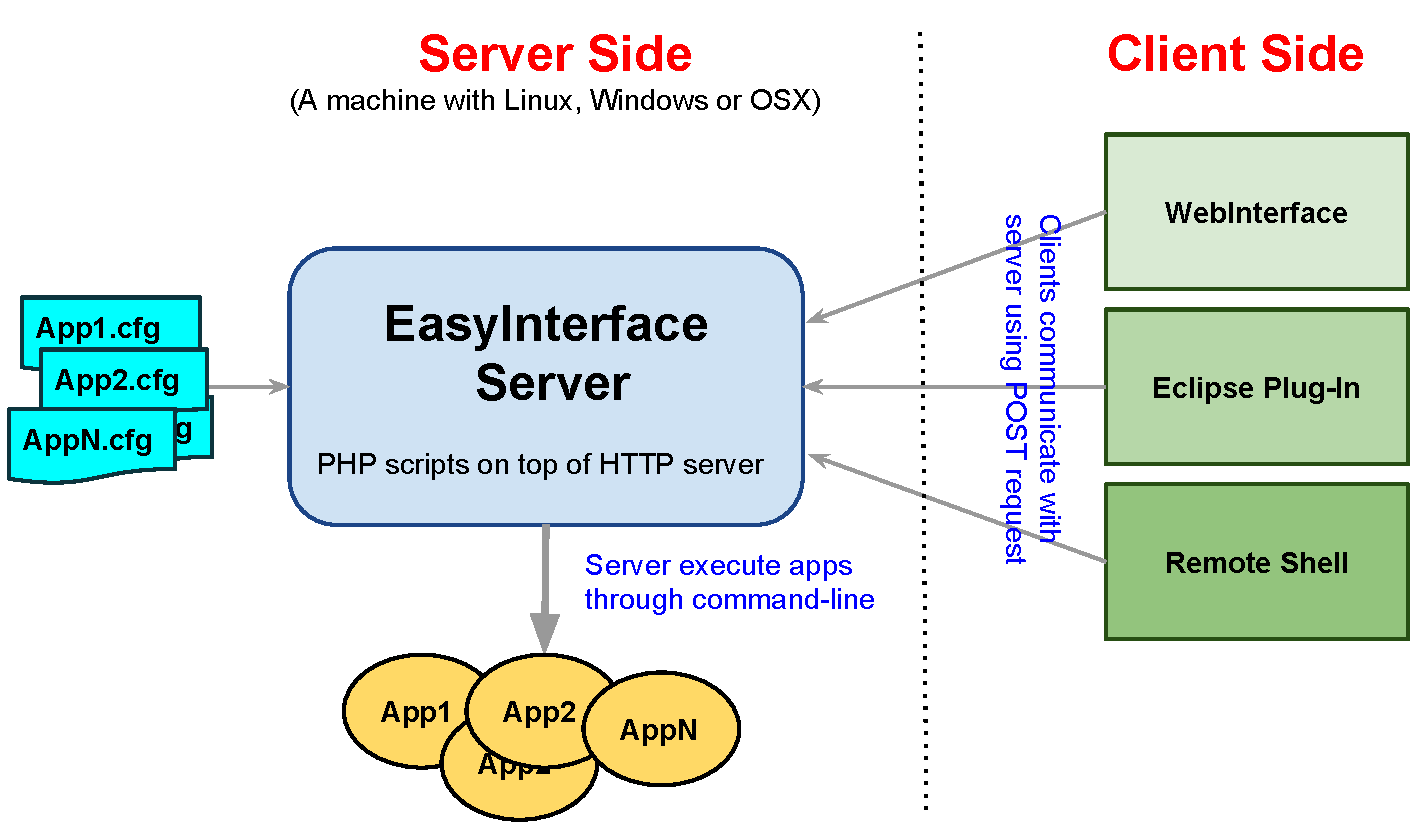
\includegraphics[width=0.5\textwidth]{fig/ei.pdf}}
\end{center}
\caption{The Architecture of the \ei Framework}
\label{fig:eiframework}
\end{figure}

The architecture of the \ei framework is depicted in
Figure~\ref{fig:eiframework}. It includes two main components:
%
(1) \emph{server side}: a machine with several applications (the
circles \texttt{App1}, \texttt{App2}, etc.) that can be executed from
a command-line and produce their output to the standard output. These
are the applications that we want to make available for the outside
world, i.e., execute them as services on the internet; and
%
(2) \emph{client side}: several clients that makes it easy to
  communicate with the server side to execute application, etc.
%
In what follows we start explaining the inner components of the server
side, and which problems they solve, and then we move on to explain the
client side.

\section{The Server Side}
\label{ch:overview:arch:server}

The problem that we want to solve at the server side is: 
%
\begin{quote}
  provide a uniform way for accessing the locally installed
  application as services (i.e., through the internet).
\end{quote}
%
This problem is solved by the \ei server, which is collection of PHP
programs that run on an HTTP server. The \ei server allows specifying
how a local applications can be executed and which parameter they take
using simple configuration files (\texttt{App1.cfg},
\texttt{App2.cfg}, etc.). For example, the following is a snippet of
such configuration file:

\medskip
\begin{lstlisting}
<app id='myapp' visible="true">
  ...
  <execinfo method="cmdline">
    <cmdlineapp>./default/myapp.sh _ei_parameters</cmdlineapp>
  </execinfo>
  <parameters prefix = "-" check="false">
    ...
    <selectone name="c">
      <option value="1" />
      <option value="2" />
    </selectone>
  </parameters>
</app>
\end{lstlisting}

\medskip
\noindent
This XML defines an application that has a unique identifier
\lst{myapp}.  The \lst{cmdlineapp} tag is a template that describes
how to execute the application from a command-line. Here
\lst{_ei_parameters} is a template parameter that will be replaced by
an appropriate value. The \lst{parameters} tag includes a list of
parameters accepted by the application. For example, there is a
parameter called ``\texttt{c}'' that can take one of the values $1$ or
$2$.
%
Once the configuration file is installed on the \ei server, anyone can
access the application using an HTTP POST request that include
something similar to the following:

\medskip
\begin{lstlisting}
{
  (*command: "execute",*)
  (*app\_id: "myapp",*)
  (*parameters:*) {
     (*c: ["1"],*)
     (*...*)
  },
  (*...*)
}
\end{lstlisting} 

\medskip
\noindent
When the \ei server receives such a request, it generates a
corresponding command-line (according to what is describe din the
configuration file), executes it, and redirect the standard output
back to the client.

\section{The Clients Side}
\label{ch:overview:arch:clients}

\begin{figure}[t]
\begin{center}
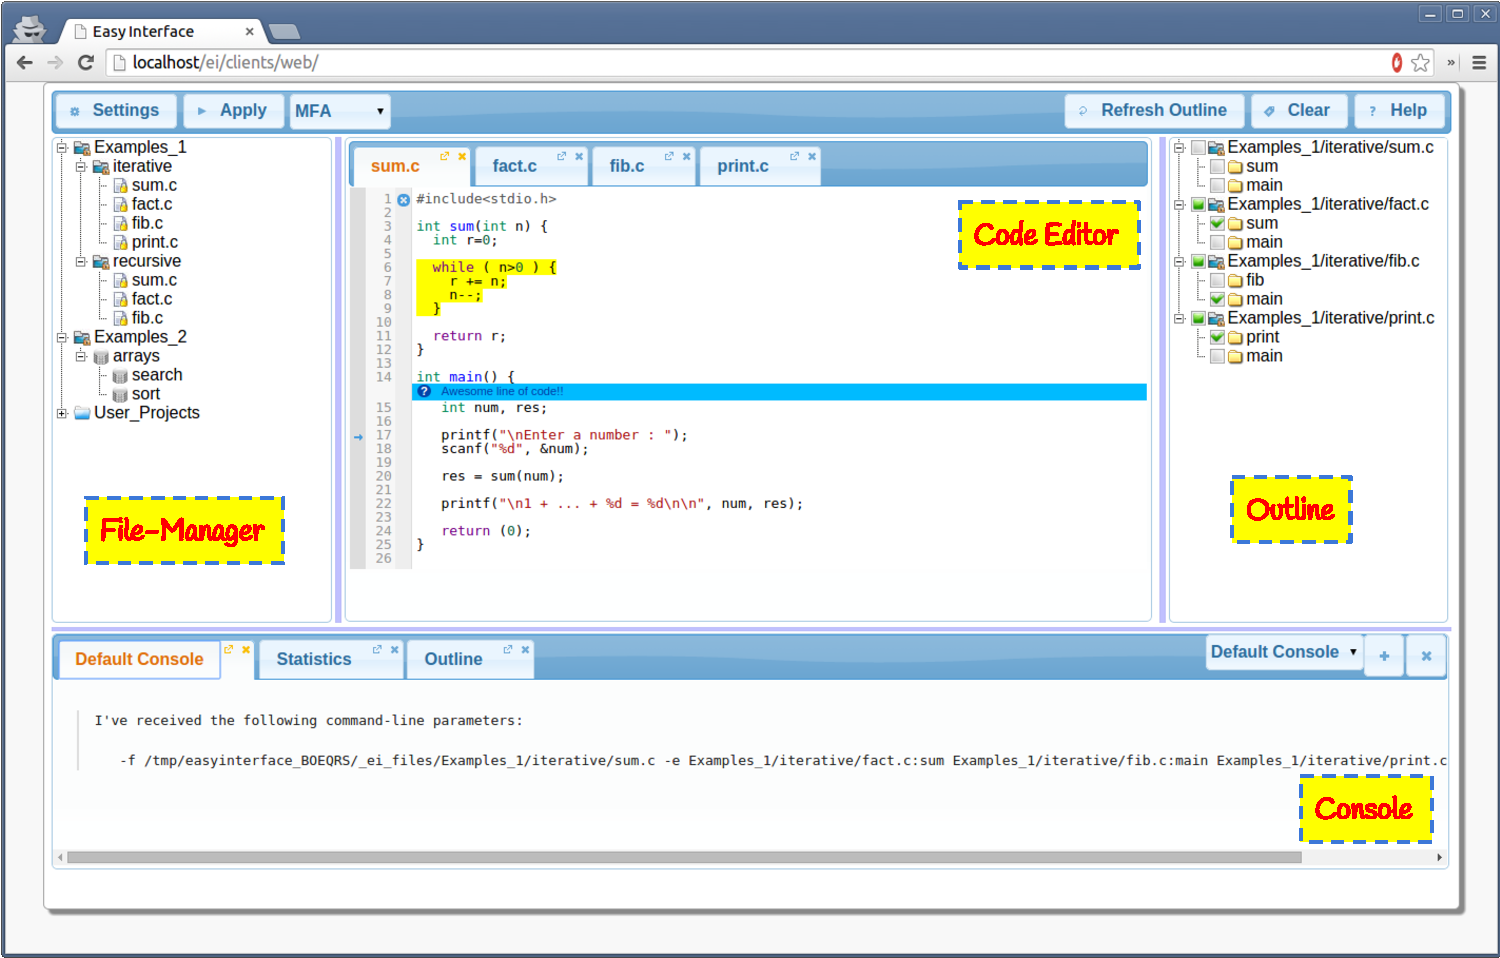
\includegraphics[width=0.95\textwidth]{fig/webclient.pdf}
\end{center}
\caption{\ei Web Client}
\label{fig:webclient}
\end{figure}

Although we now have a relatively easy way to execute applications on
the server side, it is still not as easy as we aimed at.
%
Our aim is to simplify this process further by providing (graphical)
user interfaces that automatically (1) connect to the \ei server and
ask for the list of available applications; (2) let the user choose an
application to execute and set the values of the corresponding
parameters; (3) generate a corresponding request and send it to the
\ei server; and (4) shows the returned output to the user.
%
The \ei framework provides three such interfaces: a
\emph{web-interface} that can be executed in a browser and looks like
a developing environment; an Eclipse-plugin that runs within the
Eclipse IDE; and a remote-shell that can be used from a command-line.

Since the web-client and the Eclipse plugin include are GUI based
developing environments, \ei provide also, to an application, the
possibility to generate output that has some graphical effect, e.g.,
open dialog-boxes, highlight code line, add markers, etc. To use this
feature, the applications should be modified to use the \ei output
language. The following is a snippet of such output:

\medskip
\begin{lstlisting}
<highlightlines dest="/Examples_1/iterative/sum.s"> 
  <lines> <line from="5" to="10"/> </lines>
</highlightlines>
...
<oncodelineclick dest="/Examples_1/iterative/sum.c" outclass="info" >
  <lines><line from="17" /></lines>
  <eicommands>
    <dialogbox boxtitle="Hey!"> 
      <content format="text">
       (* Click on the marker again to close this window *)
      </content>
    </dialogbox>
  </eicommands>
</oncodelineclick>

\end{lstlisting}

\medskip
\noindent
The \lst{highlightlines} indicates that lines $5--10$ of the file
\texttt{/Examples\_1/iterative/sum.s} (which is opened in the editor)
should be highlighted. The \lst{oncodelineclick} tag indicates that
when clicking on line $17$, a dialog-box with a corresponding message
should be opened.
%
Note that the application is only modified once to produce such
output, then it will have a corresponding effect in all interfaces
that support this language.





%%% Local Variables: 
%%% mode: latex
%%% TeX-master: "manual"
%%% End: 

{% -*- mode: LaTeX; TeX-PDF-mode: t; TeX-master: "manual"; -*-
}

\chapter{\ei in a Nutshell}

In this chapter we give quick introduction to \emph{integrating an
  application in the \ei framework}. In particular, we develop a
simple application, integrate it in the \ei server, and try it out
through the web-client.
%
The presentation is incremental, we start with a simple application
and in each step we add more features to demonstrate the different
parts of the \ei framework.
%
In our explanation we assume that a Unix based operating system is
used, however, we comment on how to do the analog operations on
Windows when they are different.
%
Note that in this chapter we only use the web-client, for other
clients refer to Chapter~\ref{ch:clients}.

We assume that \ei is already installed and working, which can be done
following the instructions in
``\href{http://github.com/abstools/easyinterface}{INSTALL.md}''. Thus,
if you visit \url{http://localhost/ei/clients/web} you would get a
page similar to the one shown in Figure~\ref{}. Let us start by
explaining the over all idea using the demo examples that already
available in the distribution of \ei.


In the top part of this page, you can see a button named \applybutton
and to its right a combo-box with several items named \texttt{Test-0},
\texttt{Test-1}, etc. These item correspond to applications that are
installed on the \ei server, the web-client is by default configured
to connect to the server at \url{http://localhost/ei/server} and asks
for all applications available. If you click in the \settingbutton you
will see that each application has also some parameters that can be
set to some specific values, these parameters where returned by the
server as well. If you select an application, and click on
\applybutton, the web-client sends a request to the server to execute
this application together with the values of the selected parameters
and the file that is currently active in the editor area. 
%
The serve in trun executeds the corresponding application, which is in
this case is the script \texttt{server/bin/default/test-i.sh}, and
redirect back the output to the client which will either print it in
the console, or view it graphicaly if it uses the \ei output
lagauge. Execute the demo application just to get an idea on which
output we are ta;king about.

In the rest of this chapter we explain, step by step, how to add you
own application to \ei. We do so by incrementally developing a simple
application and integrating it in the \ei server.

\section{Add Your First Application to the \ei Server}

When we add an application to the \ei server it will appear
automatically in the applications menu of the web-client (unless you
have changed the configuration of the web-client already!).
%
This is because the web-client is configured to retrieve all
applications that are installed on the server that is available at
\url{http://localhost/ei/server} (it is easy to see this in
\texttt{clients/web/index.html} at the end). Let us add a simple
``Hello World'' application.


We start by creating a bash-script that represents the executable of
our application (it could be any other executable). Create a file
named \texttt{myapp.sh} in \texttt{server/bin/default} with the
following content:

\medskip
\begin{lstlisting}[style=script]
#!/bin/bash

echo "Hello World!"
\end{lstlisting}

\medskip
\noindent
As you can see, it is just a simple program that prints "Hello World"
on the standard output. Later we will see how to pass input to this
application and how to generate more sophisticated output.
%
Change the permissions of \texttt{myapp.sh} by executing the
following:

\medskip
\begin{lstlisting}
> chmod -R 755 myapp.sh
\end{lstlisting}

\medskip
\noindent
Execute \texttt{myapp.sh} (in a shell) to make sure that it works
correctly before proceeding to the next step.

Next we will configure the server to recognize our application.
%
Create a file \texttt{myapp.cfg} in the directory
\texttt{server/config/default} with the following content:

\medskip
\begin{lstlisting}
<app visible="true">
  <appinfo>
    <acronym>MFA</acronym>
    <title>My First Application</title>
    <desc>
      <short>A simple EI application</short>
      <long>A simple application that I've done using the EasyInterface Framework</long>
    </desc>
  </appinfo>
  <apphelp>
    <content format='html'>
      This is my first <b>EasyInterface</b> application!
    </content>
  </apphelp>
  <execinfo method="cmdline">
    <cmdlineapp>./bin/myapp.sh</cmdlineapp>
  </execinfo>
</app>
\end{lstlisting}

\medskip
\noindent
Let us explain the meaning of the different elements of this
configuration file.
%
The \lst{app} tag is used to declare an \ei application, and its
\lst{visible} attribute tells the server to list this application when
someone asks for the list of installed applications. Changing this
value to \lst{"false"} will make the application ``hidden'' so only
those who know its identifier can use it.
%
The \lst{appinfo} tag provides general information about the
application, this will be used by the clients to list the application
names, etc.
%
The \lst{apphelp} tag provides some usage information about the
application, or simply redirect to another page where such information
can be found. The actual content goes inside the \lst{content} tag,
which is HTML as indicated by the \lst{format} attribute (use 'text'
for plain text).
%
The most important part is the \lst{execinfo} tag, which provides
information on how to execute the application. The attribute
\lst{method} declares that this application can be executed using a
command-line as described in \lst{cmdlineapp}.
%
The text inside \lst{cmdlineapp} is interpreted as a command-line
\emph{template}, such that when the server is requested to execute the
corresponding application it will simply execute this command-line and
redirect the output back to the client. Later you will understand why
we call it \emph{template}.

Next we add the above configuration file to the server. This is done
by adding the following line to \texttt{server/config/default/apps.cfg}
(inside the \lst{apps} tag):

\medskip
\begin{lstlisting}
 <app id="myapp" src="default/myapp.cfg" />
\end{lstlisting}

\medskip
\noindent
Here we tell the server that we want to install an application as
defined in \texttt{myapp.cfg}, and we want to assign it the
\emph{unique} identifier \lst{"myapp"}. This identifier will be mainly
used by the server and the clients when they communicate, we are not
going to use it anywhere else. 
%
Note that in \texttt{default/apps.cfg} we used
\lst{"default/myapp.cfg"} and not \lst{"myapp.cfg"}. This is because
the server looks for configurations file starting in
\texttt{server/config}.
%
Note also that the main configuration file of the \ei server is
\texttt{server/config/eiserver.cfg}, and that
\texttt{default/apps.cfg} is imported into that file (open
\texttt{server/config/eiserver.cfg} to see this).

Let us test our application. Go back to the web-client and reload the
page, you should see a new application named \texttt{MFA} in the
applications menu. If you click on the \helpbutton button you will see
the text provided inside the \lst{apphelp} tag in the \texttt{MFA}
section.
%
Select this application and click on the \applybutton button, the
message "Hello World!" will printed on the console area.


\section{Passing Input Files to Your Application}

Applications typically receive input files (e.g., programs) to
process. You must have noticed that the web-client provides the
possibility of creating and editing such files.  In this section we
explain how to pass these files, via the server, to our application
when the \applybutton button is clicked.

When you click on the \applybutton button the web-client passes the
currently opened file (i.e., the content of the active tab) to the
server, and when you use the \applybutton option from the context menu
of the filemanager\footnote{Select an element from the files tree on
  the left, and use the mouse right-click to open the context menu} it
passes all files in the corresponding sub-tree.
%
What is left is to tell the server how to pass these files to our
application. Let us assume that \texttt{myapp.sh} is prepared to
receive input files as follows:

\medskip
\begin{lstlisting}
> myapp.sh -f file1.abs file2.abs file3.abs
\end{lstlisting}

\medskip 
\noindent
In order to tell the server to pass the input files (that were
received from the client) to \texttt{myapp.sh}, open
\texttt{myapp.cfg} and change the command-line template to the
following:

\medskip
\begin{lstlisting}
<cmdlineapp>./bin/default/myapp.sh -f _ei_files</cmdlineapp>
\end{lstlisting}

\medskip
\noindent
When the server receives the files from the client, it stores them in
a temporary directory, e.g., in \texttt{/tmp}, replaces \lst{_ei_files}
by the list of their names, and then execute the resulting
command-line (now you see why we call it command-line template).
%
It is important to note that only \lst{_ei_files} changes in the above
template, the rest remain the same. Thus, the parameter
``\texttt{-f}'' means nothing to the server, we could replace it by
anything else or even completely remove it -- that depends only on how
our application is programmed to receive input files.

Let us now change \texttt{myapp.sh} to process the received files in
some way, .e.g., to print the number of lines in each file. For this,
replace the content of \texttt{myapp.sh} by the following:

\medskip
\begin{lstlisting}[style=script]
#!/bin/bash

. `dirname $0`/parse_params.sh

echo "I've received the following command-line parameters:"
echo ""
echo "  $@"

echo ""
echo "File statistics:"
echo ""
for f in $files 
do
   echo " - $f has " `wc -l $f | awk '{print $1}'` "lines"
done
\end{lstlisting}
%$

\medskip
\noindent
Let us explain the above code. 
%
At line 3 we executes an external bash-script to parse the
command-line parameters, the details are not important and all you
should know is that it leaves the list of files (that appear after
\lst{-f}) in the variable \lst{files}.
%
Lines 5-7 print the command-line parameters, just to give you an idea
how the server called \texttt{myapp.sh}, and the loop at lines 12-15
traverses the list of files and prints the number of lines in each
one.

Let us test our application. First run \texttt{myapp.sh} from a shell
passing it some existing files, just to check that it works correctly.
%
Then go back to the web-client, select \texttt{MFA} from the
applications menu, open a file from the filemanager, and finally click
the \applybutton button. Alternatively, you can also select an entry
from the filemanager and choose \applybutton from its context
menu. You should see the output of the application in the console
area.

\section{Passing Outline Entities to Your Application}

In the web-client, the area on the right is called the outline area
(see Figure~\ref{}).
%
Since \ei was designed for applications that process programs in mind,
e.g., program analysis tools, this area is typically dedicated for a
tree-view of program entities, e.g., method names, class names,
etc. 
%
The idea is that, in addition to the input files, the user will select
some of these entities to indicate, for example, where the analysis
should start from or which parts of the program to analyze.
%
Next we explain how we can pass these selected entities to an
application.

By default the web-client is configured to work with \abs programs,
and thus if you open such a program (from the filemanager) and then
click on the \refreshoutline button, you will get a tree-view of this
program entities (if you use \refreshoutline from the context menu in
the filemanager you will get a tree-view of program entities for all
files in the sub-tree).
%
Note that to generate this tree-view the web-client actually executes a
``hidden'' application that is installed on the server, but this is
not relevant to our discussion now (see Section~\ref{} for more
details).

As in the case of input files, the web-client always passes the
selected entities to the server when the \applybutton button is
clicked, and it is our responsibility to indicate how these entities
should be passed to our application. 
%
Let us assume that \texttt{myapp.sh} is prepared to receive entities
using a ``\texttt{-e}'' parameter as follows:

\medskip
\begin{lstlisting}
> myapp.sh -f file1.abs file2.abs file3.abs -e Server.send Client.receive
\end{lstlisting}

\medskip 
\noindent
In order to tell the server to pass the entities (that were received
from the client) to our application, open \texttt{myapp.cfg} and
change the command-line template to the following:

\medskip
\begin{lstlisting}
<cmdlineapp>./bin/myapp.sh -f _ei_files -e _ei_outline</cmdlineapp>
\end{lstlisting}

\medskip
\noindent
As in the case of files, before executing the above command-line the
server will replace \lst{_ei_outline} by the list of received
entities.  Let us now change \texttt{myapp.sh} to process these
entities in some way, e.g., printing them on the standard output. Open
\texttt{myapp.sh} and add the following lines at the end:

\medskip
\begin{lstlisting}[style=script]
echo ""
echo "Selected entities:"
echo ""
for e in $entities 
do
   echo "- $e"
done
\end{lstlisting}
%$

\medskip
\noindent
This code simply print the entities in separated lines. Again, the
external script \texttt{parse\_params.sh} parses the command-line and
stores the list of entities in the variable \texttt{entities}.

Go back to the web-client, select some files and entities and execute
the \texttt{MFA} application again to see the result of the last
changes. It is always recommended to check that the application works
correctly from a shell first.

\section{Passing Parameters to Your Application}

In addition to input files and outline entities, real applications
receive other parameters to control different aspects. In this section
we explain how to declare parameters in the \ei framework such that
(1) they automatically appear in the web-client (or any client) so the
user can set their values; and (2) they are passed to the application
when executed.

Let us start by modifying \texttt{myapp.sh} to accept some
command-line parameters: we add a parameter ``\texttt{-s}'' to
indicate if the received outline entities should be printed; and
``\texttt{-c W}'' that takes a value \texttt{W} to indicate what to
count in each file --- here \texttt{W} can be ``\texttt{lines}'',
``\texttt{words}'' or ``\texttt{chars}''.
%
For example, \texttt{myapp.sh} could then be invoked as follows:


\medskip
\begin{lstlisting}
> myapp.sh -f file1.abs file2.abs file3.abs -e Server.send Client.receive -s -c words
\end{lstlisting}

\medskip
\noindent
To support these parameters, change the content of \texttt{myapp.sh}
to the following:

\medskip
\begin{lstlisting}[style=script]
#!/bin/bash

. `dirname $0`/parse_params.sh

echo "I've received the following command-line parameters:"
echo ""
echo "  $@"

echo ""
echo "File statistics:"
echo ""

case $whattocount in
    lines) wcparam="-l"
    ;;
    words) wcparam="-w"
    ;;
    chars) wcparam="-m"
    ;;
esac

for f in $files 
do
    echo " - $f has " `wc $wcparam $f | awk '{print $1}'` $whattocount
done

if [ $showoutline == 1 ]; then
    echo ""
    echo "Selected entities:"
    echo ""
    for e in $entities 
    do
       echo "- $e"
    done
fi
\end{lstlisting}
%$

\medskip
\noindent
Compared to the previous script, you can notice that: we added lines
13-20 to take the value of ``\texttt{-c}'' into account when calling
\texttt{wc} at line 24; and in lines 27-35 we wrapped the loop that
prints the outline entities with a condition.
%
Note that \texttt{parse\_params.sh} sets the variable
\texttt{whattocount} to the value of ``\texttt{-c}'', and sets
\texttt{showoutline} to 1 if ``\texttt{-s}'' is provided in the
command-line and to 0 otherwise. Before proceeding to the next step,
execute the script from a shell to make sure that it works correctly.

Our goal is show these parameters in the web-client (or any other
client), so the user can select the appropriate values before
executing the application. The \ei framework provides an easy way to
do this, all we have to do is to modify \texttt{myapp.cfg} to include
a description of the supported parameters. Open \texttt{myapp.cfg} and
add the following inside the \lst{app} tag (e.g., immediately after
\lst{execinfo}):

\medskip
\begin{lstlisting}
  <parameters prefix = "-" check="false">
    <selectone name="c">
      <desc>
        <short>What to count</short>
        <long>Select the elements you want to count in each input file</long>
      </desc>
      <option value="lines">
        <desc>
          <short>Lines</short>
            <long>Count lines</long>
        </desc>
      </option>
      <option value="words">
        <desc>
          <short>Words</short>
          <long>Count words</long>
          </desc>
      </option>
      <option value="chars" >
        <desc>
          <short>Chars</short>
          <long>Count characters</long>
        </desc>
      </option>
      <default value="lines"/>
    </selectone>
    <flag name="s">
      <desc>
        <short>Show outline</short>
        <long>Show the selected outline entities</long>
      </desc>
      <default value="false"/>
    </flag>
  </parameters>
\end{lstlisting}

\medskip
\noindent
Let us explain the different elements of the above XML snippet. 
%
The tag \lst{parameters} includes the definition of all
parameters. The attribute \lst{prefix} is used to specify the symbol
to be attached to the parameter name when passed to the application,
for example, if we declare a parameter with name ``c'' the server will
pass it to the application as ``-c''. Note that this attribute can be
overridden by each parameter.
%
The attribute \lst{check} tells the server to check the correctness of
the parameters before passing them to the application, i.e., that they
are valid values, etc.
%
The tag \lst{selectone} defines a parameter with \lst{name} ``c'' that
can take one value from a set of possible ones. For example, the
web-client will view it as a ComboBox.
%
The \lst{desc} environment contains a text describing this parameter
and is used by the client when viewing this parameter graphically.
%
The \lst{option} tags define the valid values for this option, from
which one can be selected, and the \lst{default} tags defines the
default value.  The \lst{desc} environment of each \lst{option}
contains a text describing this option, e.g., the \lst{short}
description is used for the text in the corresponding ComboBox.
%
The tag \lst{flag} defines a parameter with name ``s''. This parameter
has no value, it is either provided in the command-line or not, and
its \lst{default} value is \lst{"false"}, i.e., not provided. For the
complete set of parameters supported in \ei see
\xmlstructref{parameters} in Chapter~\ref{}.

Go to the web-client, refresh the page, and click on the
\settingbutton button and look for the tab titled \texttt{MFA}.  You
will now see the parameters declared above in a graphical way where
you can set their values as well.  When you click on the \applybutton
button, the web-client will pass these parameters to the server,
however, we still have to tell the server how to pass these parameters
to \texttt{myapp.sh}. Open \texttt{myapp.cfg} and change the
\lst{cmdlineapp} template to the following:

\medskip
\begin{lstlisting}
<cmdlineapp>./bin/myapp.sh -f _ei_files -e _ei_outline _ei_parameters</cmdlineapp>
\end{lstlisting}

\medskip
\noindent
As in the case of \lst{_ei_files} and \lst{_ei_outline}, the server
replace \lst{_ei_parameters} by the list of received parameters before
executing the command-line. Execute the \texttt{MFA} application from
the web-client with different values for the parameters to see how the
output changes.

\section{Using the \ei Output Language in Your Application}

In the example that we have developed so far, the web-client simply
printed the output of \texttt{myapp.sh} in the console area. This is
the default behavior of the web-client if the output does not follow
the \ei Output Language (\eiol), which is a text-based is language
that allows generating more sophisticated output such as highlighting
lines, adding markers, etc.
%
In this section we will explain the basics of this language by
extending \texttt{myapp.sh} to use it.

An output in \eiol is an XML structure of the following form:

\medskip
\noindent
\begin{lstlisting}
<eiout> 
 <eicommands>
    $\xmlstructref{eicommand}$*
 </eicommands>
 <eiactions>
    $\xmlstructref{eiaction}$*
 </eiactions>
</eiout>
\end{lstlisting}

\medskip
\noindent
where (1) \lst{eiout} is outermost tag that includes all the output
elements; (2) \xmlstructref{eicommand}* is a list of commands to be
executed; and (3) \xmlstructref{eiaction}* is a list of actions to be
declared.
%
An \xmlstructref{eicommand} is an instruction like: \emph{print a text
  on the console}, \emph{highlight lines 5-10}, \emph{add marker at
  line 5}, etc.
%
An \xmlstructref{eiaction} is an instructions like: \emph{when the
  user clicks on line 13, highlight lines 20-25}, etc.
%
In the rest of this section we discuss some commands and actions that
are supported in \eiol, for the complete list see
Chapter~\ref{ch:eiol}.

\subsection{Printing in the Console Area}

Recall that when the \eiol is used, the web-client does not redirect
the output to the console and thus we need a command to
print in the console area.
%
The following is an example of a command that prints ``Hello World''
in the console area:

\medskip
\begin{lstlisting}
<printonconsole consoleid="1" consoletitle="Welcome">
  <content format="text">
    Hello World
  </content>
</printonconsole>
\end{lstlisting}

\medskip
\noindent
The value of the \lst{consoleid} attribute is the identifier in which
the given text should be printed (e.g., in the web-client the console
area has several tabs, so the identifier refers to one of those
tabs). If a console with such identifier does not exist yet, a new
one, with a title as specified in \lst{consoletitle}, is created. If
\lst{consoleid} is not given the output goes to the default console.
%
Inside \lst{printonconsole} we can have several \lst{content} tags
which include the content to be printed (in the above example we have
only one). The attribute \lst{format} indicates the format of the
content. In the above example it is plain 'text', other formats are
supported as well, e.g., 'html'.
%

Let us change \texttt{myapp.sh} to print the different parts of its
output in several consoles. Open \texttt{myapp.sh} and change its
content to the following:


\medskip
\begin{lstlisting}[style=script]
#!/bin/bash

. `dirname $0`/parse_params.sh

echo "<eiout>"
echo "<eicommands>"
echo "<printonconsole>"
echo "<content format='text'>"
echo "I've received the following command-line parameters:"
echo ""
echo "   $@"
echo "</content>"
echo "</printonconsole>"

echo "<printonconsole consoleid='stats' consoletitle='Statistics'>"
echo "<content format='html'>"
echo "File statistics:"
echo "<div>"
echo "<ul>"

case $whattocount in
    lines) wcparam="-l"
    ;;
    words) wcparam="-w"
    ;;
    chars) wcparam="-m"
    ;;
esac

for f in $files 
do
    echo " <li> $f has " `wc $wcparam $f | awk '{print $1}'` $whattocount "</li>"
done
echo "</ul>"
echo "</div>"
echo "</content>"
echo "</printonconsole>"

if [ $showoutline == 1 ]; then
    echo "<printonconsole consoleid='outline' consoletitle='Outline'>"
    echo "<content format='html'>"
    echo ""
    echo "Selected entities:"
    echo "<ul>"
    echo ""
    for e in $entities 
    do
      echo "<li> $e </li>"
    done
    echo "</ul>"
    echo "</content>"
    echo "</printonconsole>"
fi
echo "</eicommands>"
echo "</eiout>"
\end{lstlisting}
%$

\medskip
\noindent
The output of \texttt{myapp.sh} is give in \eiol, because at Line 5 we
start the output with the tag \lst{eiout} which we close at line 55.
%
At Line 6 we start an \lst{eicommands} tag, inside \lst{eiout}, which
we close at Line 54.
%
Inside \lst{eicommands} we have 3 \lst{printonconsole} commands:
%
the first one is generated by lines 7-13; the second by lines 15-37;
and the last one by lines 40-52.
%
Note that the first command uses the default console, while the last
two use different consoles. Note also that the content in the last two
is given in HTML. 
%
Execute \texttt{myapp.sh} in a shell first to check that it works
correctly, and then execute the \texttt{MFA} application from the
web-client to see the effect of these changes.

\subsection{Adding Markers}

Next we explain a command for adding a marker next to a code line in
the editor area. The following is an example of such command:

\medskip
\begin{lstlisting}
<addmarker dest="path" outclass="info">
  <lines>
    <line from="4" />
  </lines>
  <content format='text'>
    (*text to associated to the marker*)
  </content>
</addmarker>
\end{lstlisting}

\medskip
\noindent
The attribute \lst{dest} indicates the \emph{full path} of the file in
which the marker should be added -- the path should be exactly as
received from the web-client, we will elaborate more on this point
below when extending \texttt{myapp.sh}.
%
The attribute \lst{outclass} indicates the nature of the marker, which
can be 'info', 'error', or 'warning'. This value typically affects the
icon to be used for the marker.
%
The tag \lst{lines} includes the lines in which markers should be
added, each line is give using the tag \lst{line} where the \lst{from}
attribute is the line number~(\lst{line} can be used to define a
region in other commands, this is why the attribute is called
\lst{from}).
%
The text inside the \lst{content} tag is associated to the marker (as
a tooltip, a dialog box, etc., depending on the client).

Let us elaborate more on the value of the attribute
\lst{dest}. Suppose we have a file \texttt{prog.abs} in the
web-client, and that it is located in subtree \texttt{dir1} and then
\texttt{dir2} (i.e., in the tree-view of the filemanager starting from
the root).
%
When the web-client passes this file to the server it assigns it the
name \texttt{/dir1/dir2/prog.abs}. However, when the server passes
this file to the application it assigns it the name
\texttt{/tmp/\_ei\_filesXYZ/dir1/dir2/prog.abs}. 
%
This is because the server stores all files in the temporary directory
\texttt{/tmp/\_ei\_filesXYZ}. This temporary directory is not fixed, it
can change from one request to another, and it might vary from one
operating system to another.

When an application wants to refer to this file (e.g., for setting the
value of \lst{dest}, it must use the original name
\texttt{/dir1/dir2/prog.abs}.
%
Thus, we must know in advance that the server uses
\texttt{/tmp/\_ei\_filesXYZ} as a temporary directory so we can remove
it from \texttt{/tmp/\_ei\_filesXYZ/dir1/dir2/prog.abs} to get the
original name \texttt{/dir1/dir2/prog.abs}. 
%
We can do this by asking the server to pass the name to the temporary
directory to the application. This can be done using \lst{_ei_root} in
the command-line template, e.g., we can modify \texttt{myapp.cfg} to
the following:

\medskip
\begin{lstlisting}
<cmdlineapp>./bin/myapp.sh [...] -r _ei_root</cmdlineapp>
\end{lstlisting}

\medskip
\noindent
where \lst{[...]} stands for the template we had \texttt{myapp.cfg}
already (i.e., we just add ``\lst{-r _ei_root}'').
%
The server will change \lst{_ei_root} by the name of the temporary
directory in which the files are saved, e.g., by
\texttt{/tmp/\_ei\_fileXYZ} in the example above.

Let us modify \texttt{myapp.sh} to add a marker at Line 1 of each file
that it receives. Open \texttt{myapp.sh} and add the following code
snippet immediately before 54 of the previous script (i.e.,
immediately before closing the \lst{eicommands} tag):

\medskip
\begin{lstlisting}[style=script]
for f in $files 
do
  dest=${f#$rootdir}
  echo "<addmarker dest='$dest' outclass='info'>"
  echo "<lines><line from='1'/></lines>"
  echo "<content format='text'> text for info marker of $dest</content>"
  echo "</addmarker>"
done
\end{lstlisting}
%$

\medskip
\noindent
The code at Line 3 removes the temporary directory prefix from the file
name and stores the result in variable \texttt{dest}. Line 4-7
generate the actual command to add a marker.
%
Note that \texttt{parse\_params.sh} sets the variable \texttt{rootdir}
to the value of \lst{_ei_root} that is passed to \texttt{myapp.sh}
using the ``\texttt{-r}'' parameter.
%
Execute \texttt{myapp.sh} in a shell first to check that it works
correctly, and then execute the \texttt{MFA} application from the
web-client to see the effect of these changes.

\subsection{Highlighting Code Lines}

The following command can be used to highlight code lines:

\medskip
\begin{lstlisting}
<highlightlines dest="path" outclass="info" > 
  <lines>
    <line from="5" to="10"/>
  </lines>
</highlightlines>
\end{lstlisting}

\medskip
\noindent
Attributes \lst{dest} and \lst{outclass} are as in the \lst{addmarker}
command. Each \lst{line} tag define a region to be highlighted. E.g.,
in the above example it highlights lines 5-10. You can also use the
attributes \lst{fromch} and \lst{toch} to indicate the columns in
which the highlight start and ends respectively.

Let us modify \texttt{myapp.sh} to highlight lines 5-10 of each file
that it receives. Open \texttt{myapp.sh} and add the following code
snippet immediately before the instruction that closes the
\lst{eicommands} tag:

\medskip
\begin{lstlisting}[style=script]
for f in $files 
do
  dest=${f#$rootdir}
  echo "<highlightlines dest='$dest' outclass='info'>"
  echo "<lines><line from='5' to='10'/></lines>"
  echo "</highlightlines>"
done
\end{lstlisting}
%$

\medskip
\noindent
Execute \texttt{myapp.sh} in a shell first to check that it works
correctly, and then execute the \texttt{MFA} application from the
web-client to see the effect of these changes.

\subsection{Adding Inline Markers}

Inline markers are widgets placed inside the code. They typically
include some read-only. The following command adds an inline marker:

\medskip
\begin{lstlisting}
<addinlinemarker  dest="path" outclass="info"> 
    <lines><line from="15" /></lines>
    <content format="text">
       (* Text to be viewed in the inline marker *)
    </content>
</addinlinemarker>
\end{lstlisting}

\medskip
\noindent
Attributes \lst{dest} and \lst{outclass} are as in the \lst{addmarker}
command. Each \lst{line} tag defines a line in which a widget, showing
the text inside the \lst{content}, is added. Note that some client,
e.g., the web-client, allow only plain 'text' content.

Let us modify \texttt{myapp.sh} to add an inline marker at line 15 of
each file that it receives. Open \texttt{myapp.sh} and add the
following code snippet immediately before the instruction that closes
the \lst{eicommands} tag:

\medskip
\begin{lstlisting}[style=script]for f in $files 
do
  dest=${f#$rootdir}
  echo "<addinlinemarker dest='$dest' outclass='info'>"
  echo "  <lines><line from='15' /></lines>"
  echo "  <content format='text'> Awesome line of code!!</content>"
  echo "</addinlinemarker>"
done
\end{lstlisting}
%$

\medskip
\noindent
Execute \texttt{myapp.sh} in a shell first to check that it works
correctly, and then execute the \texttt{MFA} application from the
web-client to see the effect of these changes.


\subsection{Opening a Dialog Box}

The following command can be used to open a dialog box with some
content:

\medskip
\begin{lstlisting}
<dialogbox outclass="info" boxtitle="Done!" boxwidth="100" boxheight="100"> 
  <content format="html">
    (* text to be shown in the dialog box *)
  </content>
</dialogbox>
\end{lstlisting}

\medskip 
\noindent 
The dialog box will be titled as specified in \lst{boxtitle}, and it
will include the content as specified in the \lst{content}
environments. The attributes \lst{boxwidth} and \lst{boxheight} are
optional, they determine the initial size of the window.

Let us modify \texttt{myapp.sh} to open a dialog box with some
message. Open \texttt{myapp.sh} and add the following code snippet
immediately before the instruction that closes the \lst{eicommands}
tag:

\medskip
\begin{lstlisting}[style=script]
echo "<dialogbox outclass='info' boxtitle='Done!'  boxwidth='300' boxheight='100'>"
echo "  <content format='html'>"
echo "    The <span style='color: red'>MFA</span> analysis has been applied."
echo "    You can see the output in the result in the text area and the corresponding"
echo "    program files."
echo "  </content>"
echo "</dialogbox>"
\end{lstlisting}

\medskip
\noindent
Execute \texttt{myapp.sh} in a shell first to check that it works
correctly, and then execute the \texttt{MFA} application from the
web-client to see the effect of these changes.


\subsection{Adding Code Line Actions}

A code line action defines a list of commands to be executed when the
user clicks on a line of code (more precisely, on a marker placed next
to the line). The commands can be any of those seen above. The
following is an example of such action:

\medskip
\begin{lstlisting}
<oncodelineclick dest="/a/b/c.abs" outclass="info" >
  <lines><line from="20" /></lines>
  <eicommands>
    <highlightlines>
      <lines>
        <line from="20" to="25"/>
      </lines>
    </highlightlines>
    <dialogbox boxtitle="Hey!"> 
      <content format="html">
       (* Click on the marker again to close this window *)
      </content>
    </dialogbox>
  </eicommands>
</oncodelineclick>
\end{lstlisting}

\medskip
\noindent
First note that the above XML should be placed inside the
\lst{eiactions} tag (that we have ignored so far).
%
When the above action is executed, by the web-client for example, a
marker (typically an arrow) will be shown next to line 20 of the file
\texttt{/a/b/c.abs}.
%
Then, if the user clicks on this marker the commands inside the
\lst{eicommands} tag will be executed, and if the user clicks again
the effect of these commands is undone.
%
In the above case a click highlights lines 20-25 and will opens dialog
box, and another click removes the highlights and closes the dialog
box.
%
Note that the commands inside \lst{eicommands} inherit the \lst{dest}
and \lst{outclass} attributes of \lst{oncodelineclick}, but one can
override them, e.g., if we add \lst{dest="/a/f/p.abs"} to the
\lst{highlightlines} command then a click highlights lines 20-25 of
\texttt{/a/f/p.abs} instead of \texttt{/a/b/c.abs}.
%

Let us modify \texttt{myapp.sh} to open add a code line action, as the
one above, for each file that it receives. Open \texttt{myapp.sh} and
add the following code snippet immediately before the instruction that
closes the \lst{eiout} tag (i.e., after closing \lst{eicommands}):

\medskip
\begin{lstlisting}[style=script]
echo "<eiactions>"

for f in $files 
do
  dest=${f#$rootdir}
  echo "<oncodelineclick dest='$dest' outclass='info' >"
  echo "<lines><line from='20' /></lines>"
  echo "<eicommands>"
  echo "<highlightlines>"
  echo "<lines><line from='20' to='25'/></lines>"
  echo "</highlightlines>"
  echo "<dialogbox boxtitle='Hey!'> "
  echo "<content format='html'>"
  echo "Click on the marker again to close this window"
  echo "</content>"
  echo "</dialogbox>"
  echo "</eicommands>"
  echo "</oncodelineclick>"
done

echo "</eiactions>"
\end{lstlisting}


\medskip
\noindent
Note that at line 1 we open the tag \lst{eiactions} and at line 21 we
close it. The rest of the code simply prints a code line action as the
one above for each file.
%
Execute \texttt{myapp.sh} in a shell first to check that it works
correctly, and then execute the \texttt{MFA} application from the
web-client to see the effect of these changes.

\subsection{Adding OnClick Actions}

OnClick actions are similar to code line actions. The difference is
that instead of assigning the action to a line of code, we can assign
it to any HTML tag that we have generated.
%
For example, suppose that at some point the application has generated
the following content in the console area:

\medskip
\begin{lstlisting}
<content format="html"/>
   <span style="color: red;" id="err1">10 errors</span> were found in the file program.abs
</content>
\end{lstlisting}

\medskip
\noindent
Note that the text ``10 errors'' is wrap by a span tag with an
identifier \texttt{err1}. The OnClick action can assign a list of
commands to be executed when this text is clicked as follows.

\begin{lstlisting}
<onclick>
   <elements>
     <selector value="#err1"/>
  </elements>
  <eicommands>
    <dialogbox boxtitle="Errors"> 
      <content format="html">
       (* There are some variables used but not declated *)
      </content>
    </dialogbox>
  </eicommands>
</onclick>
\end{lstlisting}

\medskip
\noindent
It is east to see that this action is very similar to
\lst{codelineaction}, the difference is that instead of \lst{lines} we
now use \lst{elements} to identify those HTML elements a click on
which should execute the commands. 

Let us modify \texttt{myapp.sh} to open add an OnClick action assigned
to the list of files that it prints on the console. First look for the
first occurrence of 

\medskip
\begin{lstlisting}[style=script]
echo "<ul>"
\end{lstlisting}

\medskip
\noindent
which should be at line 19, and change it by

\medskip
\begin{lstlisting}[style=script]
echo "<ul style='background: yellow;' id='files'>"
\end{lstlisting}

\medskip
\noindent
This change will give the list of files that we print in the console
the identifier \texttt{files}, and will change its background color to
yellow. Next add the following code immediately before the instruction
that closes \lst{eiactions}:

\medskip
\begin{lstlisting}[style=script]
echo "<onclick>"
echo "<elements>"
echo "<selector value='#files'/>"
echo "</elements>"
echo "<eicommands>"
echo "<dialogbox boxtitle='Errors'> "
echo "<content format='html'>"
echo "There are some variables used but not declated"
echo "</content>"
echo "</dialogbox>"
echo "</eicommands>"
echo "</onclick>"
\end{lstlisting}

\medskip
\noindent
Execute \texttt{myapp.sh} in a shell first to check that it works
correctly, and then execute the \texttt{MFA} application from the
web-client to see the effect of these changes. In particular, clicking
on the list of files in the console area (anywhere in the yellow
region) should open a dialog box.

\subsection{Adding SVG Content}

\subsection{How to add examples to the file-manager}

The left side of the web-client includes several program
examples. This part is flexible and you can add you own set of
examples. You have to provide an XML that defines the examples
structure. Look for example at \texttt{server/config/example.1.cfg},
you will find the following:

\medskip
\begin{lstlisting}
<exset id="set1">
 <folder name="Examples_1">
    <folder name="PeerToPeer">
      <file name="PeerToPeer.abs" url="/ei/examples/cost/PeerToPeer.abs" />
    </folder>
    <github owner="friker92" repo="campaweb"/>
    <folder name="Cost_Centers">
      <file name="CostCenters.abs" url="/ei/examples/cost/CostCenters.abs" />
    </folder>
 </folder>
</exset>
\end{lstlisting}

\medskip
\noindent
This corresponds to the first set of example in the web client. You
can easily understand the above structure. It allows defining folders,
file, and access github repositories. If you generate your own set of
examples, e.g., \texttt{server/config/example.cfg}, you will have to
modify \texttt{examples.cfg} to include the following line:

\medskip
\begin{lstlisting}
  <exset id="set4" src="examples.3.cfg" />
\end{lstlisting}

\medskip
\indent
As for applications, the \lst{id} attribute must be unique among all
\lst{exset} defined in the same server.

By default, the web-client is configure to retrieve all examples
available on the server (see the corresponding line in
\texttt{clients/web/index.html}. This behavior can be changed (see
Section~\ref{}).

If the a URL for an example uses a domain that is different from the
one in which the web-client is installed, then make sure that the
\texttt{.htaccess} file includes the following lines:

\begin{lstlisting}
(*Header add Access-Control-Allow-Origin "*"*)
(*Header add Access-Control-Allow-Headers "origin, x-requested-with, content-type"*)
(*Header add Access-Control-Allow-Methods "PUT, GET, POST, DELETE, OPTIONS"*)
\end{lstlisting}

{% -*- mode: LaTeX; TeX-PDF-mode: t; TeX-master: "manual"; -*-
}
\chapter{\ei Server}
\label{ch:server}

This chapter describes the server side of the \ei framework, that we
refer to as the \ei server (or simply the server).
%
As explained in Section~\ref{ch:overview:arch:server}, the goal of
this server is to provide a uniform way to access local applications
and examples (i.e., those installed on the same machine where the
server runs).


The \ei server achieves the above goal by:
%
(1) providing a way to describe, using XML based configuration files,
how to execute a local application and which parameters it takes, as
well as define sets of related examples; and
%
(2) providing a JSON based protocol that can be used to request
information on those applications and examples, execute applications,
etc.
%
Section~\ref{ch:server:config} describes the syntax of the server
configuration file, which covers point~(1) above; and
Section~\ref{ch:server:protocol} describes the protocol that can be
used to communicate with the server.
%
This chapter does not cover issues related to installation, for such
documentation see
\texttt{\href{http://github.com/abstools/easyinterface}{INSTALL.md}}.


\section{Configuring the \ei Server}
\label{ch:server:config}

This section describes how to configure the \ei server.
%
Section~\ref{ch:server:config:file} explains where the configuration
file show be placed, and Section~\ref{ch:server:config:xml} describes
the (valid) content of this file.
%
Before proceeding to the next sections, it highly recommended to read
Chapter~\ref{ch:quickguide} to get a general idea on how the
configuration file looks like, etc.


\subsection{Name and Path of the Configuration File}
\label{ch:server:config:file}

By default the server looks for the configuration file
\texttt{server/config/eiserver.cfg}, and if no such file exists it
uses \texttt{server/config/eiserver.default.cfg}.
%
The default installation comes with a predefined
\texttt{sever/config/eiserver.default.cfg} that includes some demo
applications and corresponding examples. It is very recommended not
make substantial changes to \texttt{eiserver.default.cfg}, and instead
create your own \texttt{eiserver.cfg}. This way you can always have a
correct configuration file at hand from which you can copy, etc.

\subsection{The Syntax of the Configuration File}
\label{ch:server:config:xml}

The content of the configuration file should adhere to the
\xmlstructref{server}{eiserver} XML structure that is described below.
%
Inside this tag you can define applications, examples, etc. The best
way to understand how to do is follow the links in the definition of
\xmlstructref{server}{eiserver}.

\subsubsection*{General comment about XML structures} 

For the purpose of better organization of the configuration files, any
XML structure

\medskip
\begin{lstlisting}
<tagname ...>
  ....
</tagname>
\end{lstlisting}

\medskip
\noindent
can be also written as

\medskip
\begin{lstlisting}
<tagname src=$\xmlstructref{server}{cfgfilename}$ />
\end{lstlisting}

\medskip
\noindent
where the file \xmlstructref{server}{cfgfilename} includes the actual XML
structure (of the first form). However, if the XML structure has an
attribute \lst{id} then it must appear as well in the second form.

\subsubsection*{The main XML tag of the configuration file}

%% EISERVER
\bigskip
\xmlstruct
{server}
{eiserver}
{%
This XML tag is the root of the configurations file.
%
The \xmlstructref{server}{settings} section is used for setting some global
parameters; the \xmlstructref{server}{apps} section defines which applications
are available on the server; and \xmlstructref{server}{examples} defines which
sets of examples are available on the server.
%
}



\subsubsection*{General settings}

%% SETTINGS
\bigskip
\xmlstruct
{server}
{settings}
{%
%
  This tag is does not include anything yet. It is reserved for future
  use, where we plan to put general settings that are related to the
  server and not to specific application or examples set.
%
}

\subsubsection*{Examples settings}

%% EXAMPLES
\bigskip
\xmlstruct
{server}
{examples}
{%
%
  This tag is used to declare sets of examples sets that are available
  in the server, where each such set is defined by one
  \xmlstructref{server}{exset}.
%
}


%% EXSET
\bigskip
\xmlstruct
{server}
{exset}
{%
%
  This tag declare a set of examples, which are defined by collection
  of \xmlstructref{server}{exelement} (a file, a directory, or a link to a
  github repository).
%
  The attribute \xmlstructattr{id} is a unique identifier that is used
  to refer to this set when communicating with the server.
%
}


%% EXAMPLE element
\bigskip
\xmlstruct
{server}
{exelement}
{%
%
  An example element, which can be a file \xmlstructref{server}{file}, a
  folder \xmlstructref{server}{folder}, or a link to a github repository
  \xmlstructref{server}{github}.
%
}



%% File
\bigskip
\xmlstruct
{server}
{file}
{%
%
  This tags declares a file, where the \xmlstructattr{name} attribute
  is its name and \xmlstructattr{url} is a link to its content. Note
  that \xmlstructattr{name} is not necessarily the same as the one in
  \xmlstructattr{url}.
%
}


%% Folder
\bigskip
\xmlstruct
{server}
{folder}
{%
%
  This tags declares a folder with \xmlstructattr{name} as its
  name. The content of this is a list of \xmlstructref{server}{exelement}
  tags, which in turn declare the inner files, folders, etc.
%
}



%% GitHub
\bigskip
\xmlstruct
{server}
{github}
{%
%
  Declares a reference to the public github repository
  \xmlstructattr{repo} which is owned by the user
  \xmlstructattr{owner}. Optionally one can also refer to a specific
  \xmlstructattr{branch} which \texttt{master} by default, and to a
  specific \xmlstructattr{githubpath} (a directory or a single file) which
  is a the root directory by default.
%
}


\subsubsection*{Applications settings}

%% APPS
\bigskip
\xmlstruct
{server}
{apps}
{%
%
  Thhis tag declares a list of applications (to be added to the
  server). Each such application is defined by one \xmlstructref{server}{app}
  environment.  
%
} 


%% APP
\bigskip
\xmlstruct
{server}
{app}
{%
%
  This tag defines an application, where the meaning different parts
  is as follows:
%
  \begin{itemize}

  \item \xmlstructattr{id} is a unique identifier used to refer to
    this application when communicating with the server.

  \item \xmlstructattr{visible} indicates if this application should
    be listed when the list of available applications is requested ---
    by default it is \texttt{true}. 
    %
    Note that even if an application is not visible, it can be used
    like any other application by those who know it
    \xmlstructattr{id}.

  \item \xmlstructref{server}{appinfo} provides some general information about
    the application, e.g., title, logo, etc.

  \item \xmlstructref{server}{apphelp} provides enough information on how the
    application can be used, etc. It is mainly used in the help
    sections of the different clients.

  \item \xmlstructref{server}{execinfo} defines how the application can be
    executed (e.g., from a command-line).

  \item \xmlstructref{server}{parameters} defines the set parameters accepted
    by the application.

  \end{itemize}
%
}



%% APPINFO
\bigskip
\xmlstruct
{server}
{appinfo}
{%
%
  This tag provides general information for an application:
%
  \begin{itemize}
  \item \xmlstructref{server}{acronym} is an acronym for the application,
    e.g., COSTA;
  \item \xmlstructref{server}{title} is the full name of the application;
  \item \xmlstructref{server}{logo} is an image corresponding to the log of
    the application; and
  \item \xmlstructref{server}{desc} is a description of the tool.
  \end{itemize}
%
}



%% ACRONYM
\bigskip
\xmlstruct
{server}
{acronym}
{%
%
  Plain text to be used as an acronym, e.g., COSTA.
%
}



%% TITLE
\bigskip
\xmlstruct
{server}
{title}
{%
%
  Plain text deciding a title, e.g., for an application. It is
  typically more informative than an acronym (see
  $\xmlstructref{server}{acronym}$.
%
}



%% LOGO
\bigskip
\xmlstruct
{server}
{logo}
{%
%
  A link to an image --- in some standard format such
  \xmlstructvalue{png}, \xmlstructvalue{jpg} or \xmlstructvalue{gif}
  --- to be used by clients as a logo (for an application). 
%
}



%% DESC
\bigskip
\xmlstruct
{server}
{desc}
{%
%
  This is a description of some entities, e.g., of an application, a
  parameter, a parameter option, etc. It consists of two parts, the
  first one is a short description, and the second is a detailed
  description. In both cases it should be plain text. Clients will
  select one of them depending on the intended use.
%
}
{}%


%% APPHELP
\bigskip
\xmlstruct
{server}
{apphelp}
{%
%
  A (formatted) text that provides enough information on how an
  application can be used, etc. It can be provided in several formats,
  e.g., html or plain text, by using several \xmlstructref{server}{content}
  tags. Clients are supposed to pick the appropriate format if more
  than one is available. It is recommended to always include a content
  in plain text since it can be view in any client.
%
}



%% CONTENT
\bigskip
\xmlstruct
{server}
{content}
{%
%
  A text given in a specific \xmlstructattr{format}, e.g.,
  \xmlstructvalue{"text"}, \xmlstructvalue{"html"}, etc. If the
  attribute \xmlstructattr{format} is not provided, then it is assumed
  to be \xmlstructvalue{"text"} format (plain text).
%
}


%% EXECINFO
\bigskip
\xmlstruct
{server}
{execinfo}
{%
%
  Provides information on how to execute an application. Currently it
  includes only a command-line template \xmlstructref{server}{cmdlineapp}.
%
}


%% CMDLINEAPP
\noindent
\xmlstruct
{server}
{cmdlineapp}
{%
%
  Describes how to run an application, where
  \xmlstructref{server}{cmdtemplate} is a template describing a
  command-line. It is best explained by an example. Consider the
  following template example

  \bigskip
  ~~~
  \fbox{\small\texttt{/path-to/app \xmlstructtemplate{_ei_files} -m \xmlstructtemplate{_ei_outline}  \xmlstructtemplate{_ei_parameters}}}
  
  \bigskip
  \noindent
  In this template, anything that starts with \xmlstructtemplate{_ei}
  is a template parameter that will be replaced by some corresponding
  information, and \texttt{/path-to/app} is the application
  executable.
  % 
  When the server receives a request for executing the corresponding
  application, the request includes several data that should passed to
  the application. For example, the following are typical data that
  should be passed to an application:
  %
  \begin{enumerate}
  \item files to be processed (e.g., program to be analyzed);
  \item entities selected from the program outline (e.g., methods); and
  \item values for the different parameters.
  \end{enumerate}
  %
  The server passes this data to the application by replacing the
  template parameters with corresponding data as follows:
  % 
  \begin{enumerate}
  \item the files are stored locally (e.g., in \texttt{/tmp}), and
    \xmlstructtemplate{_ei_files} is replaced by a list file names
    (each with an absolute path, separated by a space);
  \item \xmlstructtemplate{_ei_outline} is replaced by a list of
    selected entities (e.g., method names); and
  \item \xmlstructtemplate{_ei_parameters} is replaced by the list of
    parameters generated from those provided in the request.
  \end{enumerate}
  % 
  This result in, for example, the following instance of the template:

  \bigskip
  \hspace{0.7cm}
  \fbox{\texttt{/path-to/app \xmlstructtemplate{a.c b.c} -m \xmlstructtemplate{a.main} \xmlstructtemplate{-v 1 -d 3 -a}}}

  \bigskip 
  \noindent
  which is then executed and its output is redirected to the
  client. The server does some security checks to guarantee that the
  command-line is not harmful. % TODO refer to the security section when available

  \bigskip 
  \noindent
  The following is a list of template parameters that can be used:

%%
  \begin{itemize}
  \item \xmlstructtemplate{_ei_files} is replaced by a list of file
    names (separated by space) in the local file system;

  \item \xmlstructtemplate{_ei_root} is replaced by the local
    temporary directory name, where all files have been saved. This
    file is of the form \texttt{/path-to-tmp/\_ei\_files} where
    \texttt{/path-to-tmp} depends on the operating system (e.g.,
    \texttt{/tmp} in Linux);
%%
  \item \xmlstructtemplate{_ei_outline} is replaced by a list of
    selected entities (separated by space);
%%
  \item \xmlstructtemplate{_ei_parameters} is replaced by a
    corresponding list of parameters (see \xmlstructref{server}{parameters});
%%
  \item \xmlstructtemplate{_ei_sessionid} is replaced by a session
    identifier, this makes it possible to track the information of a
    user along several request;
%%
  \item \xmlstructtemplate{_ei_clientid} is replaced by the client
    identifier, i.e., \texttt{webclient}, \texttt{eclipse}, etc.,
    which makes it possible to provide output depending on the
    client. See Chapter~\ref{ch:clients} for a list of clients and
    their corresponding identifiers.
  \end{itemize}
%
}


\subsubsection{Application parameters}

%% PARAMETERS
\bigskip 
\xmlstruct
{server}
{parameters} 
{%
%
  Defines a list of parameters that are accepted by a corresponding
  application. Each parameter is define by one \xmlstructref{server}{param}
  environment. 
  %
  The \xmlstructattr{prefix} attribute is used to specify a string
  that will be attached to each parameter name when passed to the
  application.
  % 
  For example, if \xmlstructattr{prefix}=\xmlstructvalue{"{-}{-}"} and
  there is a parameter called 'level' with value X, then '{-}{-}level
  X' will be passed to the application.  The default value of
  \xmlstructattr{prefix} is \xmlstructvalue{"-"}. It can also be set
  to an empty string if there is no need for a prefix.
  %
  The \xmlstructattr{check} attribute is used to indicate if the
  server should verify that the values of the parameters are valid
  (w.r.t. the specified values). The default value of
  \xmlstructattr{check} is \xmlstructvalue{"true"}.
  %
  The attributes \xmlstructattr{prefix} and \xmlstructattr{check} are
  inherited by each parameter \xmlstructref{server}{param}, which in turn can
  override then as well.
%
}
{}%

%% PARAM
\bigskip
\xmlstruct
{server}
{param}
{
%
  Defines a parameter accepted by a corresponding application. There
  are several types of parameters supported:
\begin{itemize}
\item \xmlstructref{server}{selectone} defines a parameter that takes one
  value from a predefined set;
\item \xmlstructref{server}{selectmany} defines a parameter that takes several
  values from a predefined set;
\item \xmlstructref{server}{flag} defines a parameter that either appear or
  not in the command-line; and
\item \xmlstructref{server}{textfield} defines a parameter that take a
  free-text value.
\end{itemize}
%
}


%% SELECTONE
\bigskip
\xmlstruct
{server}
{selectone}
{%
%
  Defines a parameter that takes a \emph{single} value out of a given
  list:

  \begin{itemize}
  \item \xmlstructattr{name} is the name of the parameter, it must be
    unique among all parameters of an app;

  \item \xmlstructattr{prefix} and \xmlstructattr{check} can be used
    to override the corresponding attributes of
    \xmlstructref{server}{parameters};

  \item \xmlstructref{server}{desc} provide a description of this parameter;

  \item \xmlstructref{server}{option}+ is a list of possible values for
    this parameter;

  \item \xmlstructref{server}{defaultvalue} specifies the default value. If
    not specified then the first \xmlstructref{server}{option} is considered
    as the default one;

  \item \xmlstructattr{widgetid} specifies the preferred layout when
    used in a client with a graphical interface (e.g., combo-box,
    radio button, etc.). This is client depends, see
    Chapter~\ref{ch:clients} for more information.

  \end{itemize}
%
}


%% SELECTMANY
\bigskip
\xmlstruct
{server}
{selectmany}
{%
%
  Defines a parameter that takes \emph{several} values out of a given
  list. The meaning of the attributes and inner environments is as in
  \xmlstructref{server}{selectone}, except that in this case we can specify
  several  \xmlstructref{server}{defaultvalue}.
%
}


%% FLAG
\bigskip
\xmlstruct
{server}
{flag}
{%
%
  Defines a parameter that can take \texttt{true} or \texttt{false}
  values. The meaning of the attributes and inner environments is as
  in \xmlstructref{server}{selectone}. In addition, the attribute
  \xmlstructattr{explicit} is used to specify how this parameter
  should be passed to the application. For example, assume the
  parameter name is \texttt{f}, then:
  % 
  \begin{itemize}
  %  
  \item when \xmlstructattr{explicit} is \xmlstructvalue{true} the
    parameter is explicitly passed to the application, i.e., using
    ``\texttt{-f true}'' or ``\texttt{-f false}''; and
  %
  \item when \xmlstructattr{explicit} is \xmlstructvalue{false}
    parameter is passed as ``\texttt{-f}'' if its value is
    \texttt{true} and not passed at all if its value is
    \texttt{false}.
  % 
  \end{itemize}
%
  The default value of \xmlstructattr{explicit} is
  \xmlstructvalue{false}.
%
}


%% TEXTFIELD
\bigskip
\xmlstruct
{server}
{textfield}
{%
%
  Defines a parameter that can take free-text value. The meaning of
  the attributes and inner environments is as in
  \xmlstructref{server}{selectone}. The \lst{initialtext} tag includes a text
  to be shown in the corresponding text-area by default.  The meaning
  of extra attributes is as follows:
%
\begin{itemize}
%
\item \xmlstructattr{multiline} is used to specify if the free-text
  should be single-line or multi-lines. By default its values is
  \xmlstructvalue{false}, i.e., single-line.
%
\item \xmlstructattr{passinfile} is used to indicate that the actual
  value should be saved into a file, and what is passed to the
  application is the file name instead of the actual text. 
  % 
  This should be used for safety, when there is a risk that the
  free-text can be harmful to the command-line (although the server
  does some checks to avoid this).
%
\end{itemize}
}


%% OPTION
\bigskip
\xmlstruct
{server}
{option}
{%
Defines an option (i.e., a possible value) for a parameter.
}


%% Default value
\bigskip
\xmlstruct
{server}
{defaultvalue}
{%
Defines a default value for a parameter.
}



\bigskip
\noindent
\xmlstructdef{server}{textformat}

( \lst{"text"} | \lst{"html"} | \lst{"svg"})

\bigskip
\noindent
\xmlstructdef{server}{paramvalue}

[a-z,A-Z,0-9,-,\_]+

\bigskip
\noindent
\xmlstructdef{server}{paramname}

[a-z,A-Z,0-9,-,\_]+

\bigskip
\noindent
\xmlstructdef{server}{bool}

( \lst{"true"} | \lst{"false"} )

\bigskip
\noindent
\xmlstructdef{server}{appid}

[a-z,A-Z,0-9,-,\_]+

\bigskip
\noindent
\xmlstructdef{server}{exsetid}

[a-z,A-Z,0-9,-,\_]+

\bigskip
\noindent
\xmlstructdef{server}{widgetid}

[a-z,A-Z,0-9,-,\_]+

\bigskip
\noindent
\xmlstructdef{server}{url}

A valid \texttt{http} or \texttt{https} URL.

\bigskip
\noindent
\xmlstructdef{server}{paramprefix}

Can be any string that matches [a-z,A-Z,0-9,-,\_]+, typically
\lst{"-"} or \lst{"--"}.

\bigskip
\noindent
\xmlstructdef{server}{text}

Free text.

\bigskip
\noindent
\xmlstructdef{server}{githubpath}

A path to a file or a directory in a github repository (relative to
the root of the repository).

\bigskip
\noindent
\xmlstructdef{server}{githubbranch}

A valid branch name for a github repository.

\bigskip
\noindent
\xmlstructdef{server}{githubuser}

A valid github username.

\bigskip
\noindent
\xmlstructdef{server}{githubrepo}

A valid github repository.

\bigskip
\noindent
\xmlstructdef{server}{foldername}

[a-z,A-Z,0-9,-,.,\_]+

\bigskip
\noindent
\xmlstructdef{server}{filename}

[a-z,A-Z,0-9,-,.,\_]+

\bigskip
\noindent
\xmlstructdef{server}{cfgfilename}

A path to a configuration file. Should be relative to
\texttt{server/config}.

\bigskip
\noindent
\xmlstructdef{server}{cmdtemplate}

The explanation is given in \xmlstructref{server}{cmdlineapp}

\section{Communicating with the \ei Server}
\label{ch:server:protocol}

This section describes the protocol to be user for communicating with
the \ei server. If you are not developing any \ei client, then this
section is not relevant for you.

The \ei server is a collection of PHP scripts running on top of an
HTTP server. Communicating with the server is done through HTTP POST
requests. In particular, the request should be assigned to a POST
attribute called ``\texttt{eirequest}'' (the actual value of
``\texttt{eirequest}'' is a JSON record that we will described in
the next sections). The following is an example of how one can
communicate with the server using JavaScript:

\bigskip
\begin{lstlisting}
var req = ...; // the actual JSON record of the request
$\$$.post("http://localhost/ei/server/eiserver.php",
{
  eirequest: req
},
function(data) { 
  // do something with data
});
\end{lstlisting}

\bigskip
\noindent
The response of the server is an XML of the following form:

\bigskip
\begin{lstlisting}
<ei_response>
  <ei_server_output> ...  </ei_server_output>
  <ei_output> ... </ei_output>
  <ei_error> ... </ei_error>
</ei_response>
\end{lstlisting}

\bigskip
\noindent
Where
%
\begin{itemize}
%
\item \lst{ei_server_output} includes messages printed by
  server. These messages are not the response to the request, but
  rather debugging messages that can be useful when developing
  clients, etc.
%
\item \lst{ei_output} includes the response to the request, i.e., if
  we request to execute an application the output of that application
  goes inside this tag.
%
\item \lst{ei_error} includes error messages that are related to the
  request.
%
\end{itemize}
%
Typically, \lst{ei_output} and \lst{ei_error} are mutually exclusive,
i.e., only one can appear in the response.

\bigskip 
In the next section we describe how the format of the request for
driving information on applications, execute and application, and
retrieve example sets.

\subsection{Retrieve Information on Available Applications}

To retrieve information on a given application, or all visible
applications on the server, use the following request:

\bigskip
\begin{lstlisting}
{
  command: CMD,
  app_id: ID
}
\end{lstlisting}

\bigskip
\noindent
where (1) \texttt{CMD} is \texttt{app\_info},
\texttt{app\_parameters}, or \texttt{app\_details}; and (2)
\texttt{ID} is either the special value \texttt{\_ei\_all} (i.e., all
applications) or an application identifier as specified in
\xmlstructref{server}{app}.
%
A successful request will return (inside the \lst{ei_output} tag) the
XML structure \xmlstructref{server}{apps} (that is defined in the
configuration file) after filtering out some information as we explain
next.
%
First any application that does not match \texttt{ID} is removed (if
\texttt{ID} is \texttt{\_ei\_all} then only non-visible applications
are removed). Then, for any remaining applications:
%
\begin{itemize}
%
\item if \texttt{CMD} equals \texttt{app\_info}, it returns only the
  \xmlstructref{server}{appinfo} of each application;
%
\item if \texttt{CMD} equals \texttt{app\_parameters}, it returns only the
  \xmlstructref{server}{parameters} of each application; and
%
\item if \texttt{CMD} equals \texttt{app\_details}, it returns
  everything except \xmlstructref{server}{execinfo} of each
  application.
%
\end{itemize}
%
Note that \xmlstructref{server}{execinfo} is never returned as it
reveals information on how to execute an application locally.



\subsection{Execute an Application}

Next we describe, by mean of an example, the form of a request for
executing an application. Suppose we are interested in executing an
application with identifier \texttt{myapp} where, in addition, we
would like to pass it some values for the parameters, files to
process, outline entities, and the identified of the client who is
making the request. Such a request has the following form:

\bigskip
\begin{lstlisting}
{
  command: (*"execute"*),
  app_id: (*"myapp"*),
  (*parameters*): {
    (*"l"*): (*[ "true" ]*),
    (*"f"*): (*[ "false" ]*),
    (*"s"*): (*[ "yes" ]*),
    (*"x"*): (*[ "1", "2" ]*), 
    (*"\_ei\_clientid"*): (*"webclient"*),
    (*"\_ei\_outline"*): (* [ "ent1", "ent2", ... ]*),
    (*"\_ei\_files"*): [
                  {
                    (*path*): (*"dir1"*),
                    (*type*): (*"dir"*),
                  },
                  {
                    (*path*): (*"dir2/file1.c"*),
                    (*type*): (*"text"*),
                    (*content*): (*"This is the content of dir2/file1.c"*)
                  },
                  {
                    (*path*): (*"dir2/file2.c"*),
                    (*type*): (*"text"*),
                    (*content*): (*"This is the content of dir2/file2.c"*)
                  },
                  {
                    (*path*): (*"dir3/file1.c"*),
                    (*type*): (*"text"*),
                    (*content*): (*"This is the content of dir3/file1.c"*)
                  }
                ]
  }
}
\end{lstlisting}

\bigskip
\noindent
Let us explain the different parts of this request: 
%
\begin{itemize}
%
\item \texttt{command} must have the value \texttt{``execute''};
%
\item \texttt{app\_id} should refer to the identifier of the
  application that we want to execute (it can be visible or not);
%
\item \texttt{parameters} is a JSON record that includes all the
  information, e.g., application parameters and files, that we want to
  pass to over, as we explain below.
\end{itemize}
%
Before explaining the details of the parameter records, it is
recommend that your refresh you memory with the details of the
command-line template as described
in~\xmlstructref{server}{cmdlineapp}. The parameters JSON record
includes the following information:
%
\begin{itemize}
%
\item \emph{Application parameters:} any field (of the JSON record)
  whose name does not start with \texttt{\_ei} is a parameter that is
  supposed to be defined in the \xmlstructref{server}{parameters}
  environment of the corresponding application. The value of such
  field is a list of elements that represent the value of the
  parameter. If the parameter is supposed to take a single value then
  list must have a single element.
%
\item \emph{Files}: the field \texttt{\_ei\_files} represent the files
  that we want to pass to the application. Its value is an array of
  JSON records where each record represent a text file or a directory
  (binary files are not supported yet). The \texttt{path} field of the
  record refers to the file or directory name, it is relative to the
  root of the temporal directory where the server saves these
  files. The \texttt{type} field indicates the type of the file. In
  the case of text files, the field \texttt{content} represent the
  actual content of the file.
%
\item \emph{Outline entities}: the filed \texttt{\_ei\_outline} is a
  list of elements representing thee selected entities from the
  outline.
%
\item \emph{Client identifier}: the field \texttt{\_ei\_clientid}
  indicates the identifier of the client who has performed the
  request.
%
\end{itemize}



\subsection{Retrieve Example Sets}

To retrieve the example sets use the following request:

\bigskip
\begin{lstlisting}
{
  command: "exset_details",
  app_id: ID
}
\end{lstlisting}

\bigskip
\noindent
where \texttt{ID} is either the special value \texttt{\_ei\_all}
(i.e., all example sets) or an examples set identifier as specified in
\xmlstructref{server}{exset}.
%
A successful request will return (inside the \lst{ei_output} tag) the
XML structure \xmlstructref{server}{examples} (that is defined in the
configuration file) after filtering out those example sets that do not
match the value of \texttt{ID}, i.e, if \texttt{ID} is
\texttt{\_ei\_all} then it returns all example sets, otherwise only
the indicated one.

{% -*- mode: LaTeX; TeX-PDF-mode: t; TeX-master: "manual"; -*-
}

\chapter{\ei Clients}
\label{ch:clients}

This chapter describes the different clients available in the \ei
framework. Currently the only mature one is the web-client that we
describe in Section~\ref{ch:clients:web}. The Eclipse and remote shell
clients are under development.

\section{The Web-Client}
\label{ch:clients:web}

\begin{figure}[h]
\hrule\smallskip
\begin{center}
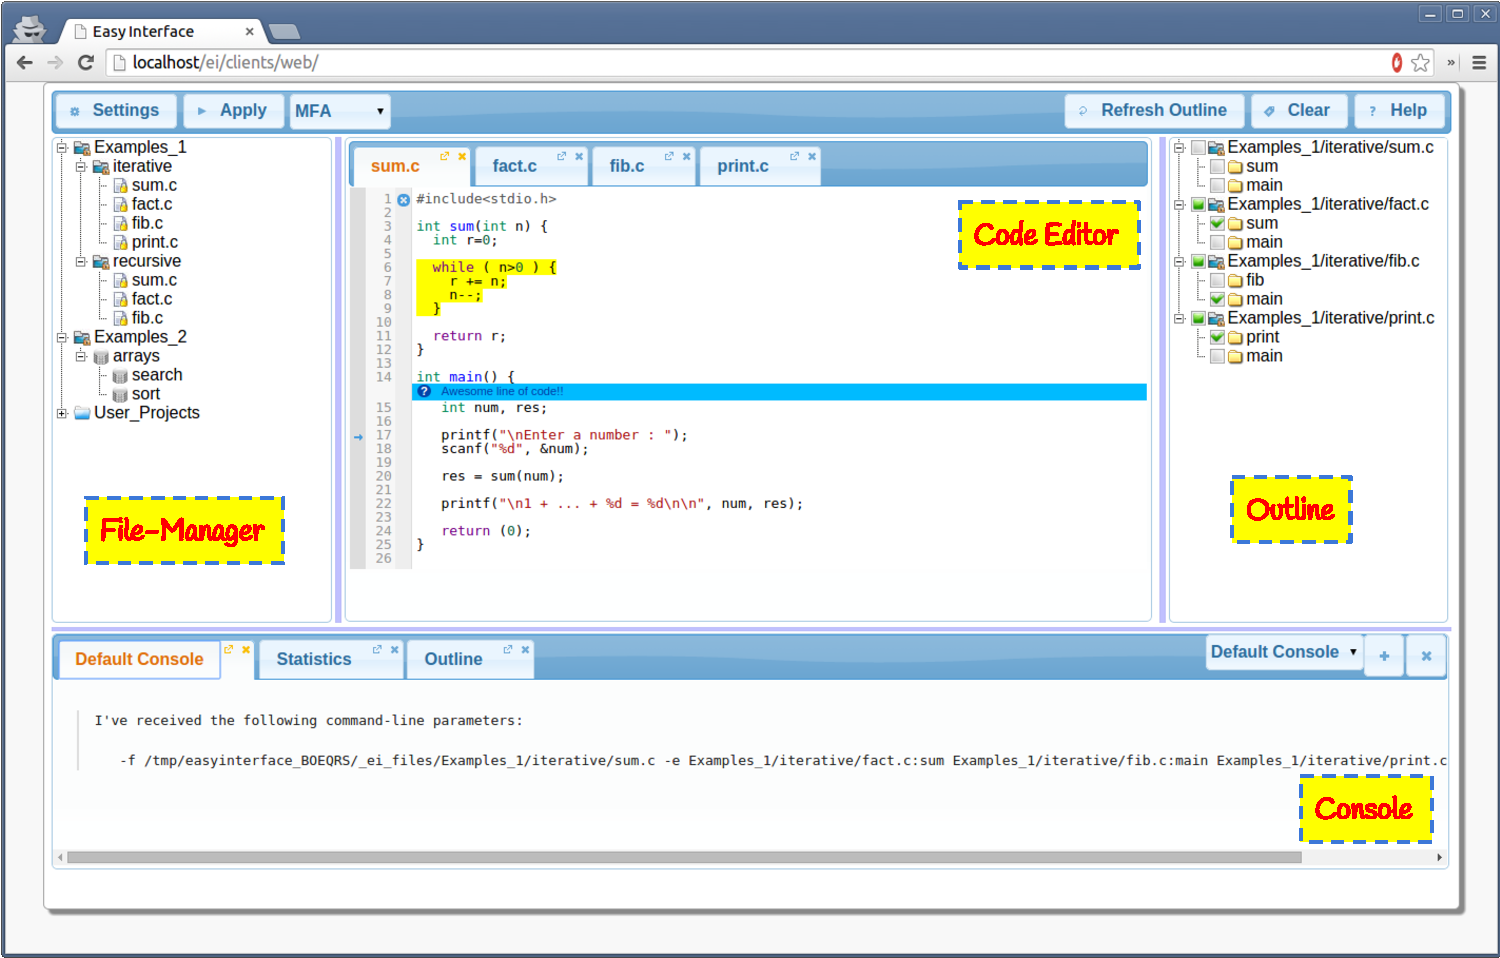
\includegraphics[width=1\textwidth]{fig/webclient.pdf}
\end{center}
\caption{\ei Web Client}
\label{fig:webclient}
\hrule
\end{figure}

The web-client of \ei is a JavaScript program that runs in a web
browser. To access it simply visit
\url{http://localhost/ei/clients/web} and you will get a page similar
to that of Figure~\ref{fig:webclient}.
%
This page has 5 main components: (1) the code area, where users can
edit programs; (2) the file-manager that contains a list of predefined
examples as well as user files; (3) the outline that includes an
outline of one or more files; (4) the console area where the results of
executing an application is printed; (5) the tools bar that includes
several buttons to execute an application, etc.

The web-client can be configured to fit your needs, it has a
configuration file to control (1) which applications to include in the
applications menu; (2) which examples to show in the file-manager; and
(3) how to generate the outline for a set of programs.
%
The web-client first looks for the configuration file
\texttt{clients/web/webclient.cfg}, and if it does not exists it uses
\texttt{clients/web/webclient.default.cfg}.
%
It is recommended not to substantially change
\texttt{webclient.default.cfg}, and instead create your own
\texttt{webclient.cfg}.
%
Next we explain the different components of the configuration file. In
what follows, when we refer the \emph{default server} we mean the one
that is available at the same address as web-client, i.e., if the
web-client was accessed using the URL
``\lst{http://somedomain/.../ei/client/web}'' then the URL of the
default server is ``\lst{http://somedomain/.../ei/server}''.

The configuration file is a text file that includes a single JSON
record with several fields. Let us explain it using the following
complete record:

\bigskip
\begin{lstlisting}
{
  (*title*): (*"Easy Interface"*),
  (*apps*): (*[\{server: "http://domain/.../ei/server, apps: ["myapp", "costa", "mhp"]\}, ... ]*),
  (*examples*): (*[\{server: "http://domain/.../ei/server, examples: ["mhpex","costex"]\}, ... ]*),
  (*outlineserver*): (*"http://domain/.../ei/server"*),
  (*outlineapp*): (*"coutline"*)
}
\end{lstlisting}

\bigskip
\noindent
All fields in the above record are optional, the web-client assigns
default values for those that are not available. 
%
The field \texttt{title} is used to set the window title (see
Figure~\ref{fig:webclient}), where its default value is ``Easy
Interface''. The field \texttt{apps} is used to change the set of
application to be listed in the applications menu, it is explained in
Section~\ref{ch:clients:web:appsmenu}. The field \texttt{examples} is
used to change the set of examples that are shown in the file-manager,
it is explained in Section~\ref{ch:clients:web:filemanager}. The
fields \texttt{outlineserver} and \texttt{outlineapp} are used to
indicate which application to use for generating the content of the
outline, it is explained in Section~\ref{ch:clients:web:outline}.

\subsection{The Applications Menu}
\label{ch:clients:web:appsmenu}

The application menu, the combo-box next to the \applybutton button in
Figure~\ref{fig:webclient}, includes a list of applications that can
be executed by the user. This list can be modified by setting the
value of the filed \texttt{apps} in the configuration file. This value
is a list of JSON records of the form

\bigskip
\begin{lstlisting}
  { (*server: SRV, apps: APPSLIST*) }
\end{lstlisting}
 
\bigskip
\noindent  
where \lst{SVR} is a URL to an \ei server and \lst{APPSLIST} is a list
of application identifiers (see \xmlstructref{server}{app}).
%
\lst{APPSLIST} can also be the special value \lst{_all} which refers
to all application of the corresponding server.
%
The default value of this field is a list with a record that refers to
all applications of the default server.

\subsection{The File-Manger}
\label{ch:clients:web:filemanager}

In the file-manager area, of Figure~\ref{fig:webclient}, you can see a
tree-view that represents programs on which the applications can be
applied, etc. The one with the name \texttt{User\_Projects}
corresponds to programs that are created by the user; and the rest are
predefined set of examples. This set of example can be modified by
setting the value of the field \texttt{examples} in the configuration
file.  This value is a list of JSON records of the form

\bigskip
\begin{lstlisting}
  { (*server: SRV, examples: EXLIST*) } 
\end{lstlisting}

\bigskip
\noindent
where \lst{SVR} is a URL to an \ei server and \lst{EXLIST} is a list
of example set identifiers (see
\xmlstructref{server}{exset}). \lst{EXLIST} can also be the special
value \lst{_all} which refers to all example sets of the corresponding
server. The default value of this field is a list with a record that
refers to all example sets of the default server.

\subsection{The Outline}
\label{ch:clients:web:outline}

The outline area of Figure~\ref{fig:webclient} includes a tree-view
that represents information on some programs, e.g., methods, classes,
etc. The actual values in this tree and its structure depend very much
on the intended use of \ei, and thus, it is completely configurable.
%
The idea is that the user will select some of the entries in this
tree, and then they will be passed to the application that we apply
(see Section~\ref{ch:quickguide:outline}
and~\xmlstructref{server}{cmdlineapp}).

The actual content of the outline is not generated by the web-client,
but rather by an external application that is installed on some \ei
server that we refer to as the \emph{outline application}. It like any
other application but typically non-visible.  The exact work-flow for
generating an outline is as follows:
%
\begin{enumerate}

\item the user clicks on the \refreshoutline button to generate an
  outline for the currently opened tab (in the code editor), or select
  the \refreshoutline option from the context menu of the file-manager
  to generate an outline for all programs in the corresponding
  sub-tree;

\item the web-client request to execute the \emph{outline
    application}, passing it all files of interest;

\item the \emph{outline application} process the input files and
  generates some XML structure that represents the content of the
  outline;

\item the web-client converts this XML into a tree view as shown in
  Figure~\ref{fig:webclient}.

\end{enumerate}
%
The fields \texttt{outlineserver} and \texttt{outlineapp} in the
configuration file can be used to indicate which application to use
for generating the outline content. The default value of
\texttt{outlineserver} is the default server, and the one of
\texttt{outlineapp} is \texttt{coutline}. As for the outline content,
it is \emph{a sequence of XML environments} that adhere to the
following syntax, each element (i.e., tree) in this sequence will be
show at the root level in the outline area:

%% 
\bigskip
\xmlstruct
{webclient}
{outline}
{%
%
  Defines a tree that represent (part of) an outline. The outer
  \lst{category} tag is the root of this tree, and the inner
  \xmlstructref{webclient}{outline}* are its children. The meaning of
  the different attributes is as follows:
%
\begin{itemize}
  \item \xmlstructattr{text} is the text to be show for that node.
  \item \xmlstructattr{value} is the value to passed to an application if that node is selected.
  \item \xmlstructattr{selectable} indicates if this node can be
    selected. Its default value is \xmlstructvalue{true}. Such nodes
    are used to divide the tree in several logical categories.  
    %
    Note that, in some clients, nodes might be still selectable even
    if the value is \xmlstructvalue{false}, however, in such case they
    will not be passed to the application.
  \item \xmlstructattr{icon} is a URL to an alternative icon to be
    used for that node.
\end{itemize}
%
\bigskip
\noindent
\xmlstructdef{webclient}{nodetext}

A string.

\bigskip
\noindent
\xmlstructdef{webclient}{nodeval}

[a-z,A-Z,0-9,-,\_,:,.]+

\bigskip
\noindent
\xmlstructdef{webclient}{bool}

( \lst{"true"} | \lst{"false"} )

\bigskip
\noindent
\xmlstructdef{webclient}{url}

A valid \texttt{http} or \texttt{https} URL.
}



\section{Eclipse Plugin}
\label{ch:clients:eclipse}

Under development. 

\section{Remote shell}
\label{ch:clients:shell}

Under development. 

{% -*- mode: LaTeX; TeX-PDF-mode: t; TeX-master: "manual"; -*-
}

\chapter{The \ei Output Language}
\label{ch:eiol}

In this chapter we describe a text-based output language that allows
tools to view their output in a graphical way, e.g., highlighting
lines, adding markers, defining on-click actions, etc. The main
advantage of this language is that it does not require any knowledge
on GUI or WEB programming.
%
Some clients, e.g., the web-client described in
Section~\ref{sec:clients:web}, are supposed to support this
language. This is done by developing a corresponding interpret that
renders the effect of the corresponding commands in the respective
environment (e.g., a web browser).

The rest of this chapter is organized as follows: 
%
in Section~\ref{sec:eiol:overview} we first give a general overview of
the design of this language; 
%
in Section~\ref{sec:eiol:spec} we describe the syntax and semantics of
this language; 
%
in Section~\ref{sec:eiol:other} we include some details that we left
out of Section~\ref{sec:eiol:spec} for readability (we refer the
reader to these parts in Section~\ref{sec:eiol:spec}); and 
%
in Section~\ref{sec:eiol:examples} we give some examples to the
different parts of the language.



\section{General Overview}
\label{sec:eiol:overview}

The idea behind the \ei output language is that a tool should just
print, on the standard output, how it wants to view the output using
some high-level description, and leave the details to an interpreter
that converts this description to graphical output.
%
This way we move the complexity of constructing a GUI from the tool to
the interpreter, and thus free developers of tools from mastering any
WEB or GUI related libraries.
%
To simplify the processing of such output, we should use some
structured format. In our case we opt for XML, but we could use any
other structured formatting. e.g., JSON.


The \ei output language assumes that the environment in which it is
interpreted includes:
%
\begin{enumerate}[\upshape(\itshape i\upshape)]

\item A ``\texttt{Code Editor}'' where programs can be edited,
  typically a tab for each file;
%
\item A ``\texttt{File Manager}'' that includes a tree-view of all
  user files and predefined examples;
%
\item A \texttt{Console} where output can be printed in different
  formats (it might include also several consoles, e.g., several
  tabs).
\end{enumerate}
%
An output in the \ei output language is an XML structure of the
following form:

\medskip
\noindent
\begin{lstlisting}
<eiout> 
 <eicommands>
    $\xmlstructref{eiout}{eicommand}$*
 </eicommands>
 <eiactions>
    $\xmlstructref{eiout}{eiaction}$*
 </eiactions>
</eiout>
\end{lstlisting}

\medskip
\noindent
where
\begin{enumerate}[\upshape(\itshape i\upshape)]
\item \lst{eiout} is the outermost tag that encapsulates all commands
  and actions;
\item \xmlstructref{eiout}{eicommand}* is a list of commands to be
  executed; and
\item \xmlstructref{eiout}{eiaction}* is a list of actions to be
  declared. Actions correspond to interactions with the user.
\end{enumerate}
%
Typical examples of \xmlstructref{eiout}{eicommand} are: \emph{print a
  text on the console}, \emph{highlight lines 5-10}, \emph{add marker
  at line 5}, etc.
%
Typical examples of \xmlstructref{eiout}{eiaction} are: \emph{when the
  user clicks on line 13, highlight lines 20-25}, \emph{when the user
  clicks on some text, open a dialog box with some message}, etc.

In the next section we give a detailed specification of this
language. Note that currently the language includes some commands and
actions of interest, that we needed for our tools in the \envisage
project, however, it is design in a way that is easily extensible to
include more commands an actions (interpreters on the client side
should be modified to support such extensions).

\section{Syntax and Semantics}
\label{sec:eiol:spec}


An output in the \ei output language is an XML structure that adhere
to the syntax of \xmlstructref{eiout}{eiout} that is described
below. You can follow the links in its definition in order to get the
definitions of its different parts. 
%
The semantics of each is fully specified, and when needed we refer the
reader to clarifying examples.

\bigskip
\noindent
\textbf{IMPORTANT:} note that the output must be a valid XML
structure, thus, in what follows, whenever we need to include
\emph{plain text} in that output, such text should be enclosed in a
\lst{<![CDATA[ $\mbox{the-text-goes-here}$ ]]>} environment (see
Example~\ref{sec:eiol:examples:4}).


%% EIOUT
%%
\bigskip
\xmlstruct
{eiout}
{eiout} 
{%
%
  This is the main environment of the output, it includes several
  lists of command environments \xmlstructref{eiout}{eicommands}, and
  several lists of action environments \xmlstructref{eiout}{eiactions}.
%
  Commands are executed first, in the given order, and then actions are
  executed in the given order as well.
%
  The \xmlstructattr{version} attribute indicates the version of the
  output language that is used, which is $1.0$ by default.
%
}


%% EICOMMANDS
%% 
\bigskip
\xmlstruct
{eiout}
{eicommands}
{%
%
A list of commands to be performed.
%
The attribute \xmlstructattr{dest} is the destination file on which
the command is applied (if needed), it should be the full path to that
file as provided by the \ei server.
%
E.g., when highlighting a line we might want to highlight a line in
one file or another. 
%
If \xmlstructattr{dest} is not specified, then the commands will be
applied to the file that is currently active, e.g., if the client
includes a code editor with several tabs, one for each file, the
command will be applied to the active tab. If none is active then the
behavior is not specified.
% 
The attribute \xmlstructattr{outclass} specifies the \emph{output
  class} of the commands in this environment, that is, the nature of
the corresponding output generated by the commands, e.g., error,
information, warning, etc. The effect of this attribute is not fully
specified and it depends on the client and the actual implementation
of the interpreter.
%
All commands inside this environment inherit the values of
\xmlstructattr{outclass} and \xmlstructattr{dest}, and each can
override them.
%
}


%% EIACTIONS
%% 
\bigskip
\xmlstruct
{eiout}
{eiactions}
{%
%
  A a list of actions to be declared. An action typically executes a
  list of \xmlstructref{eiout}{eicommands} when the user interacts with the
  interface in some predetermined way, e.g., \emph{when the user
    clicks on line 30, highlight lines number 12 and 16}. We say the
  an action is \emph{performed} as a response to the user interaction.
%
  If the user interacts again with the interface, according to what is
  specified in the action, then the action is \emph{unperformed} if
  possible (when the corresponding commands support the \emph{undo}
  operation), e.g., in the above example if the user clicks again on
  Line 30 again, the highlights of lines 12 and 16 are turned off.

  Before \emph{performing} an action, the last \emph{performed} action
  is \emph{unperformed} first. This behavior can be disabled by
  setting the \xmlstructattr{autoclean} attribute to
  \xmlstructvalue{``false''}. All actions inside this environment
  inherit the value of \xmlstructattr{autoclean}, and each can
  override it.
% 
  The attribute \xmlstructattr{dest} and \xmlstructattr{outclass} are
  as in the case of commands (see the description of
  \xmlstructref{eiout}{eicommands}).
%
}


%% EICOMMAND
%% 
\bigskip
\xmlstruct
{eiout}
{eicommand}
{
A command in the \ei output language, briefly:
\begin{itemize}
\item \xmlstructref{eiout}{printonconsolecommand} can be used to print on the console.
%
\item \xmlstructref{eiout}{highlightlinescommand} can be used to highlight
  lines in the code editor.
%
\item \xmlstructref{eiout}{dialogboxcommand} can be used to open a dialog
  window with a corresponding message.
%
\item \xmlstructref{eiout}{writefilecommand} can be used to add a file (and a
  corresponding content) to the file-manager.
%
\item \xmlstructref{eiout}{setcsscommand} can be used to change the
  CSS properties of some elements that were previously generated
  (e.g., content in HTML)
%
\item \xmlstructref{eiout}{addmarkercommand} can be used to add a marker next
  to a line in the code editor.
%
\item \xmlstructref{eiout}{addinlinemarkercommand} can be used to add a line
  widget (an inlined marker) in the code editor.
%
%% \item \xmlstructref{eiout}{streamcommand} can be used to notify that
%%   there is an stream application running.
%
\item \xmlstructref{eiout}{downloadcommand} can be used to download a
  file that was previously generated by a tool.
%
\item \xmlstructref{eiout}{changecontentcommand} can be used to modify
  a content that has been previously generated.
%
\end{itemize}
}


%% EIACTION
%% 
\bigskip
\xmlstruct
{eiout}
{eiaction}
{%
An action in the \ei output language, briefly:
\begin{itemize}
%
\item \xmlstructref{eiout}{oncodelineclickaction} can be used to perform an action
  when the user clicks on a line in the code editor.
%
\item \xmlstructref{eiout}{onclickaction} can be used to perform an
  action when the user clicks on a previously generated text (a DOM
  element in general).
%
%% \item \xmlstructref{eiout}{timelineaction} TO-DO.
%
\end{itemize}
}


%% PRINTONCONSOLECOMAND
%%
\bigskip
\xmlstruct
{eiout}
{printonconsolecommand}
{%
%
  Prints the content described by the \xmlstructref{eiout}{content}
  environments on the console that has an identifier
  \xmlstructattr{consoleid}.
%
  If \xmlstructattr{consoleid} is not specified, the output goes to
  the default console.
%
  If \xmlstructattr{consoleid} is specified but there is no console
  with such an identifier, the console is created and
  \xmlstructattr{consoletitle} (if specified) is used as its title.
%
  The attribute \xmlstructattr{outclass} is as described in
  \xmlstructref{eiout}{eicommands}.
%
  \\\\See Example~\ref{sec:eiol:examples:1}.
} 

%% HIGHLIGHTLINESCOMMAND
%%
\bigskip
\xmlstruct
{eiout}
{highlightlinescommand}
{%
%
  Highlights the lines specified by \xmlstructref{eiout}{lines} in the
  file \xmlstructattr{dest}. The attribute \xmlstructattr{outclass} is
  as described in \xmlstructref{eiout}{eicommands}.
%
  \\\\See Example~\ref{sec:eiol:examples:2}.
}

%% DIALOGBOXCOMMAND
%%
\bigskip
\xmlstruct
{eiout}
{dialogboxcommand}
{%
  Opens a dialog box with the content specified by the
  \xmlstructref{eiout}{content} environments. The value of
  \xmlstructattr{boxtitle}, if specified, is used as a title for the
  dialog box. The attributes \xmlstructattr{boxwidth} and
  \xmlstructattr{boxheight} can be used to set the size of the window.
  The attribute \xmlstructattr{outclass} is as in
  \xmlstructref{eiout}{eicommands}.
%
  \\\\See Example~\ref{sec:eiol:examples:3}.
}


%% WRITEFILECOMMAND
%%
\bigskip 
\xmlstruct 
{eiout}
{writefilecommand} 
{%
%
  Creates a new file it in the file-manager, using the path specified
  by \xmlstructattr{filename}. The file's content is set to the value
  of \xmlstructref{eiout}{text}. If the file exists, and
  \xmlstructattr{overwrite} is \xmlstructvalue{true}, the content is
  replaced otherwise a new file is created with a new name. The
  default value of \xmlstructattr{overwrite} is
  \xmlstructvalue{false}.
% 
%  This command does not support \emph{undo}.
%
  \\\\See Example~\ref{sec:eiol:examples:4}.
}


%% SETCSSCOMMAND
%%
\bigskip
\xmlstruct
{eiout}
{setcsscommand}
{%
%
  Changes the CSS properties, as specified by
  \xmlstructref{eiout}{cssproperties}, of all elements that match the
  selectors in \xmlstructref{eiout}{elements}.
%
  There must be exactly one \xmlstructref{eiout}{elements} environment and
  one \xmlstructref{eiout}{cssproperties} environment. 
%
  The elements are selected from those that were previously generated
  by other commands.
%
  \\\\See Example~\ref{sec:eiol:examples:5}.
}

%% CHANGECONTENTCOMMAND
%%
\bigskip
\xmlstruct
{eiout}
{changecontentcommand}
{%
% 
  Modifies the content of all elements that match the selectors in
  \xmlstructref{eiout}{elements}, using
  \xmlstructref{eiout}{content}. These elements are typically selected
  from those generated by previously executed commands.
%
  The attribute \xmlstructattr{action} indicates how to incorporate
  \xmlstructref{eiout}{content} in the current one, i.e.,
  \xmlstructvalue{replace}, \xmlstructvalue{append} or
  \xmlstructvalue{prepend}.
%
  \\\\See Example~\ref{sec:eiol:examples:6}.
}

%% ADDMARKERCOMMAND
%%
\bigskip
\xmlstruct
{eiout}
{addmarkercommand}
{%
%
  Adds a marker next to each line that is specified in
  \xmlstructref{eiout}{lines}. The column information from each
  \xmlstructref{eiout}{line} in \xmlstructref{eiout}{lines} is
  ignored.  All markers are associated with the content given by the
  \xmlstructref{eiout}{content} environments, as a tooltip for
  example. If the client allows expanding the tooltip to a dialog
  window, the attributes \xmlstructattr{boxtitle},
  \xmlstructattr{boxwidth} and \xmlstructattr{boxheight} can be used
  to set the properties of the corresponding window (see
  \xmlstructref{eiout}{dialogboxcommand}).
%
  If a line is already associated with a marker, then all
  \xmlstructref{eiout}{content} environments should be appended to the
  current content.
%
  The attributes \xmlstructattr{dest} and \xmlstructattr{outclass} are
  as described in \xmlstructref{eiout}{eicommands}.
%
  \\\\See Example~\ref{sec:eiol:examples:7}.
}

\bigskip
\xmlstruct
{eiout}
{addinlinemarkercommand}
{%
%
  Adds an inline marker (a line widget) for each line that is
  specified by \xmlstructref{eiout}{lines}. All line widgets will
  include the content specified by the \xmlstructref{eiout}{content}
  environments. The column information from each
  \xmlstructref{eiout}{line} in \xmlstructref{eiout}{lines} is
  ignored.
%
  If a line is already associated with a marker, then all
  \xmlstructref{eiout}{content} environments should be appended to the
  current content.
%
  The attributes \xmlstructattr{dest} and \xmlstructattr{outclass} are
  as described in \xmlstructref{eiout}{eicommands}.
%
  \\\\See Example~\ref{sec:eiol:examples:8}.
}

%% STREAM COMMAND
%% \bigskip
%% \xmlstruct
%% {eiout}
%% {streamcommand}
%% {%
%% %
%%   Notify that there is an application running and you can get their
%%   results each \xmlstructattr{time} seconds asking to the ei server
%%   with the \xmlstructattr{execid} given.
%%   %
%%   Also the \xmlstructref{eiout}{content} of the command will be
%%   printed on the console \xmlstructattr{consoleid} that print all the
%%   stream data. 
%% %
%% }

%% DOWNLOADCOMMAND
%%
\bigskip
\xmlstruct
{eiout}
{downloadcommand}
{%
%
  When a tool that runs on an \ei server X generates this command, the
  effect should be downloading the file specified in
  \xmlstructattr{filename}, from the \ei server X, using the execution
  identifier \xmlstructattr{execid}. See
  sections~\ref{sec:server:config:workflow} and
  \ref{sec:server:access:download} for more information on downloading
  files from an \ei server.
%
  \\\\See Example~\ref{sec:eiol:examples:9}.
}

%% ONCODELINECLICKACTION
%%
\bigskip
\xmlstruct
{eiout}
{oncodelineclickaction}
{%
%
  Adds (special) markers at the code lines specified by
  \xmlstructref{eiout}{lines}, such that when any is clicked the
  commands in \xmlstructref{eiout}{eicommands} are performed, and if
  clicked again they are unperformed (see detailed description in
  \xmlstructref{eiout}{eiactions}).
  % 
  The content given by the \xmlstructref{eiout}{content} environments is
  associated with the markers (as a tooltip for example).
%
  If a line is already associated with such an action, then
  \xmlstructref{eiout}{content} should be appended to the current
  content and \xmlstructref{eiout}{eicommands} should be accumulated
  to the current ones.
%
  The attributes \xmlstructattr{dest}, \xmlstructattr{outclass} and
  \xmlstructattr{autoclean} are as described in
  \xmlstructref{eiout}{eiactions}. Moreover, the
  \xmlstructref{eiout}{eicommands} environment inherits the
  \xmlstructattr{dest} and \xmlstructattr{outclass} attributes of this
  environment.
%
  \\\\See Example~\ref{sec:eiol:examples:2}.
}%

\bigskip
\xmlstruct
{eiout}
{onclickaction}
{%
%
  A click on any element that matches any selector from
  \xmlstructref{eiout}{elements} will execute the commands declared in
  \xmlstructref{eiout}{eicommands}, and if clicked again they are
  unperformed (see detailed description in
  \xmlstructref{eiout}{eiactions}).
%
  If the element is already associated with an action, then
  \xmlstructref{eiout}{eicommands} should be accumulated to the
  current ones.
%
%
  The attributes \xmlstructattr{dest}, \xmlstructattr{outclass} and
  \xmlstructattr{autoclean} are as described in
  \xmlstructref{eiout}{eiactions}. Moreover, the above
  \xmlstructref{eiout}{eicommands} environment inherits the
  \xmlstructattr{dest} and \xmlstructattr{outclass} attributes of this
  environment.
%
  \\\\See Example~\ref{sec:eiol:examples:5}.
}%

%% \bigskip
%% \xmlstruct
%% {eiout}
%% {timelineaction}
%% {%
%% %
%%   TO-DO
%% %
%% }

%% %%
%% \bigskip
%% \xmlstruct
%% {eiout}
%% {step}
%% {%
%% step of timeline
%% }


%% 
\bigskip
\xmlstruct
{eiout}
{lines}
{%
%
A group of lines, typically used to specify the lines affected by 
an \xmlstructref{eiout}{eicommand} or an \xmlstructref{eiout}{eiaction}.
%
}


%% 
\bigskip
\xmlstruct
{eiout}
{line}
{%
%
  A region (of lines) typically used to specify the region on which
  the effect of an \xmlstructref{eiout}{eicommand} or an
  \xmlstructref{eiout}{eiaction} is applied:
%
\begin{itemize}
\item \xmlstructattr{from} is the start line.
\item \xmlstructattr{to} is the end line.
\item \xmlstructattr{fromch} is the character (i.e., column number)
  where the first line starts.
\item \xmlstructattr{toch} is the character (i.e., column number)
  where the last line ends.
\end{itemize}
%
The default value of \xmlstructattr{to} is as the value of
\xmlstructattr{from}. The default value of \xmlstructattr{fromch} is
0, and of \xmlstructattr{toch} is the end of the line.
%
}


\bigskip
\xmlstruct
{eiout}
{elements}
{%
  Set of selectors (of DOM elements)
} 

\bigskip
\xmlstruct
{eiout}
{selector}
{%
%
  The attribute \xmlstructattr{value} must be a valid selector as in
  jQuery (see \url{https://jquery.com}). It is used to match some DOM
  elements.
%
}


\bigskip
\xmlstruct
{eiout}
{cssproperties}
{%
%
A set of CSS properties.
%
}


\bigskip
\xmlstruct
{eiout}
{cssproperty}
{%
%
  A CSS property. The attributes \xmlstructattr{name} and
  \xmlstructattr{value} should correspond to valid CSS properties.
%
}


%% CONTENT
\bigskip
\xmlstruct
{eiout}
{content}
{%
%
  A text \xmlstructref{eiout}{text} given in a specific
  \xmlstructattr{format}, that is supposed to be viewed to the
  user. If the attribute \xmlstructattr{format} is not provided, then
  it is assumed to be in \xmlstructvalue{"text"} format (plain text).
%
  This content should be viewed to the user in the specified
  format. The supported formats are:
%
\begin{itemize}
\item \xmlstructvalue{"text"}, for plain text;
\item \xmlstructvalue{"html"}, for HTML;
\item \xmlstructvalue{"svg"}, for Scalable Vector Graphics~\cite{svg}; and
\item \xmlstructvalue{"graph"}, for drawing 2D graphs -- see
  Section~\ref{sec:eiol:other:graph} for the exact
  format.
\end{itemize}
%
The rest of attributes can be used to associate the content with an
output stream as follows (first see
sections~\ref{sec:server:config:workflow} and
\ref{sec:server:access:stream} to understand the notions behind
streaming before you continue):
%
\begin{itemize}
\item \xmlstructattr{execid} is the execution identifier;
\item \xmlstructattr{ext} is the extension of output chunk files to be
  retrieved;
\item \xmlstructattr{action} indicates how to incorporate new output
  chunks to the current content (i.e., \xmlstructvalue{replace},
  \xmlstructvalue{append} or \xmlstructvalue{prepend}); and
\item \xmlstructattr{refreshrate} is a time interval (in seconds) to
  be used for refreshing the output. If the value is not specified
  then refreshing the output should be on demand.
\end{itemize}
%
The client should stop refreshing when the background processes of the
corresponding stream have terminated, or when the user asks to stop
them explicitly.
%
}%

\bigskip
\noindent
\xmlstructdef{eiout}{consoleid}

( [a-z,A-Z,0-9,-,\_]+ | \lst{$\mbox{new}$} | \lst{$\mbox{default}$} )

\medskip
\noindent
The value \lst{$\mbox{new}$} means a new console, we cannot refer to
this console later. The value \lst{$\mbox{default}$} means the default
console of the client.


\bigskip
\noindent
\xmlstructdef{eiout}{execid}

 [a-z,A-Z,0-9,-,\_]+

\bigskip
\noindent
\xmlstructdef{eiout}{path}


A path to a file, including the file name. There are two forms, the
first one is a full path including the temporal directory name that is
created by the server, e.g.,
``\texttt{/tmp/easyinterfae\_XYZ/\_ei\_files/dir1/dir2/file.c}''.  The
client should simply ignore the prefix
``\texttt{/tmp/easyinterfae\_XYZ/\_ei\_files/}'', i.e., the value in
this case is ``\texttt{dir1/dir2/file.c}''.  The second form does not
include the temporal directory prefix.

\bigskip
\noindent
\xmlstructdef{eiout}{file} 

A file name, without the path. Substrings \lst{"/"}, \lst{"\"}, and
\lst{".."} are not allowed.


\bigskip
\noindent
\xmlstructdef{eiout}{version}

$x.y$, where $x$ is the major version number and $y$ is the minor one,
e.g. $1.0$, $1.1$, etc.

\bigskip
\noindent
\xmlstructdef{eiout}{outclass}

( \lst{none} | \lst{info} | \lst{warning} | \lst{error} )

\bigskip
\noindent
\xmlstructdef{eiout}{bool}

( \lst{true} | \lst{false} )

\bigskip
\noindent
\xmlstructdef{eiout}{int}

An integer

\bigskip
\noindent
\xmlstructdef{eiout}{string}

A string

\bigskip
\noindent
\xmlstructdef{eiout}{text}

Free text.

\bigskip
\noindent
\xmlstructdef{eiout}{textformat}

( \lst{$\mbox{text}$} | \lst{html} | \lst{svg} | \lst{graph} )

\bigskip
\noindent
\xmlstructdef{eiout}{cssname}

A valid name for a CSS property.

\bigskip
\noindent
\xmlstructdef{eiout}{cssval}

A valid value for a corresponding CSS property.

\bigskip
\noindent
\xmlstructdef{eiout}{position}

( \lst{prepend} | \lst{append} | \lst{replace} )



\section{Other Details}
\label{sec:eiol:other}

\subsection{The Graph Format}
\label{sec:eiol:other:graph}

The \xmlstructref{eiout}{content} tag, of the \ei output language,
supports drawing $2D$ graphs using the value \xmlstructvalue{graph}
for the \xmlstructattr{format} attribute. In this section we describe
the syntax of such graphs.

Let us start by defining the notion of a graph we are discussing in
this section.  A function is a list of pairs $(x,y)$ that defines some
points in the plane, and a plot of such a function is a drawing that
connects these points.
%
A $2D$ graph is a collection of functions that share all $x$ points,
i.e., we can imagine it as drawing several functions using the same
$xy$-axes.
%
For the sake of compact representation, if we have $n$ functions,
every point in a graph can be represented as $(x,y_1,\ldots,y_n)$
where $(x,y_i)$ corresponds to the $i$-th function.

A graph is a sequence of JSON records where each record describes a
graph via the following fields:
%
\begin{itemize}
\item \lst{$\mbox{"title"}$}: a title to be used for the graph;
%
\item \lst{$\mbox{"x-title"}$}: a title to be used for the $x$-axes
  (horizontal);
%
\item \lst{$\mbox{"y-title"}$}: a title to be used for the $y$-axes
  (vertical);
%
\item \lst{$\mbox{"f-titles"}$}: an array of strings, where the $i$-th
  string is a title for the $i$-th function.
%
\item \lst{$\mbox{"values"}$}: an array of points, where each point is
  an array $[x,y_1,\ldots,y_n]$ such that $(x,y_i)$ corresponds to a
  point defining the $i$-th function.
%
\end{itemize}
%
In addition, since the \xmlstructref{eiout}{content} tag can define
several graphs, we also provide the possibility of grouping graphs
into logical groups and assigning them labels.
%
Clients should allow viewing graphs of interest as follows: a graph is
viewed if it belongs to at least one of the selected groups and has at
least one of the selected labels. 
%
Defining groups and labels is done using the following fields in the
corresponding JSON record:
%
\begin{itemize}
\item \lst{$\mbox{"groups"}$}: array of groups, where each group is
  simply a string.
\item \lst{$\mbox{"labels"}$}: array of labels, where each label is
  simply a string.
\end{itemize}
%
See Example~\ref{sec:eiol:examples:3} for an example of $2D$ graphs.


\section{Examples}
\label{sec:eiol:examples}

In this section we give some examples for the different commands and
actions of the \ei output language. Note that they are referred to
from the definitions of the corresponding commands in
Section~\ref{sec:eiol:spec}.

{% -*- mode: LaTeX; TeX-PDF-mode: t; TeX-master: "manual"; -*-
}

\begin{example}
\label{sec:eiol:examples:1}
%
The following is an example of
\xmlstructref{eiout}{printonconsolecommand} using different
\xmlstructref{eiout}{content} environments with different formats:

\medskip
\begin{lstlisting}
<printonconsole consoleid="1" consoletitle="Welcome">
  <content format="text">
    Hello World
  </content>
  <content format="html">
    <span style="color: red;">Hello</span> World
  </content>
  <content format="svg">
    <svg height="100" width="100">
      <circle cx="50" cy="50" r="40" fill="red" />
    </svg> 
  </content>
</printonconsole>
\end{lstlisting}

\medskip
\noindent
Its execution in the web-client generates the output depicted in
Figure~\ref{fig:examples:1}.

\begin{figure}[h]
\hrule\smallskip
\begin{center}
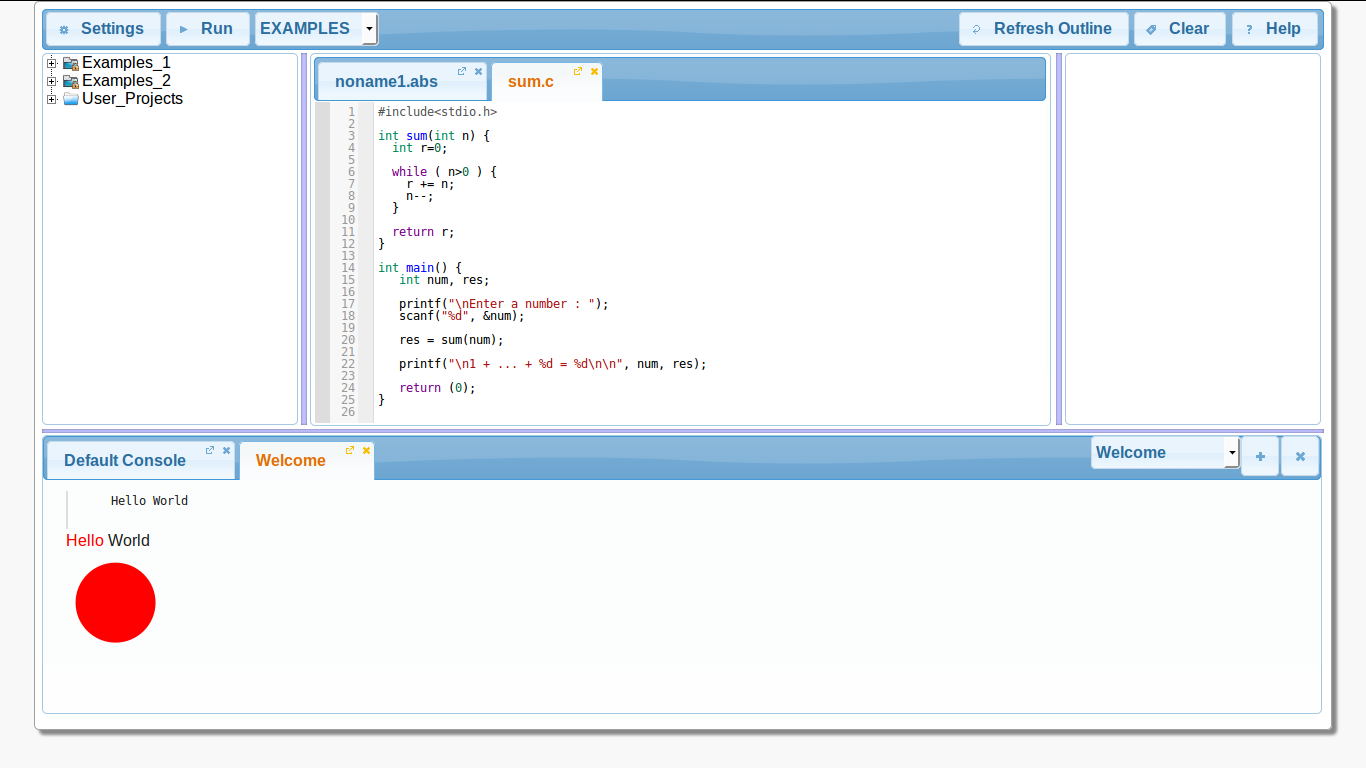
\includegraphics[width=1\textwidth]{fig/example1.png}
\end{center}
\caption{Output of Example~\ref{sec:eiol:examples:1}}
\label{fig:examples:1}
\hrule
\end{figure}
\end{example}

\begin{example}
\label{sec:eiol:examples:2}
%
The following is an example of
\xmlstructref{eiout}{oncodelineclickaction} which executes two
\xmlstructref{eiout}{highlightlinescommand}, each with different
\xmlstructattr{outclass}:

\medskip
\begin{lstlisting}
<eiactions>
 <oncodelineclick>
  <lines> <line from="3" /> </lines>
  <eicommands>
   <highlightlines outclass="info">
    <lines> <line from="2" to="4" /> </lines>
   </highlightlines>
   <highlightlines outclass="warning">
    <lines> <line from="6" fromch="4" toch="8" /> </lines>
   </highlightlines>
  </eicommands>
 </oncodelineclick>
</eiactions>
\end{lstlisting}

\medskip
\noindent
Its execution in the web-client generates the output depicted in
Figure~\ref{fig:examples:2}. Note that a click on the arrow (in the
left-side gutter) executes the commands and another click undo their
corresponding effect.


\begin{figure}[h]
\hrule\smallskip
\begin{center}
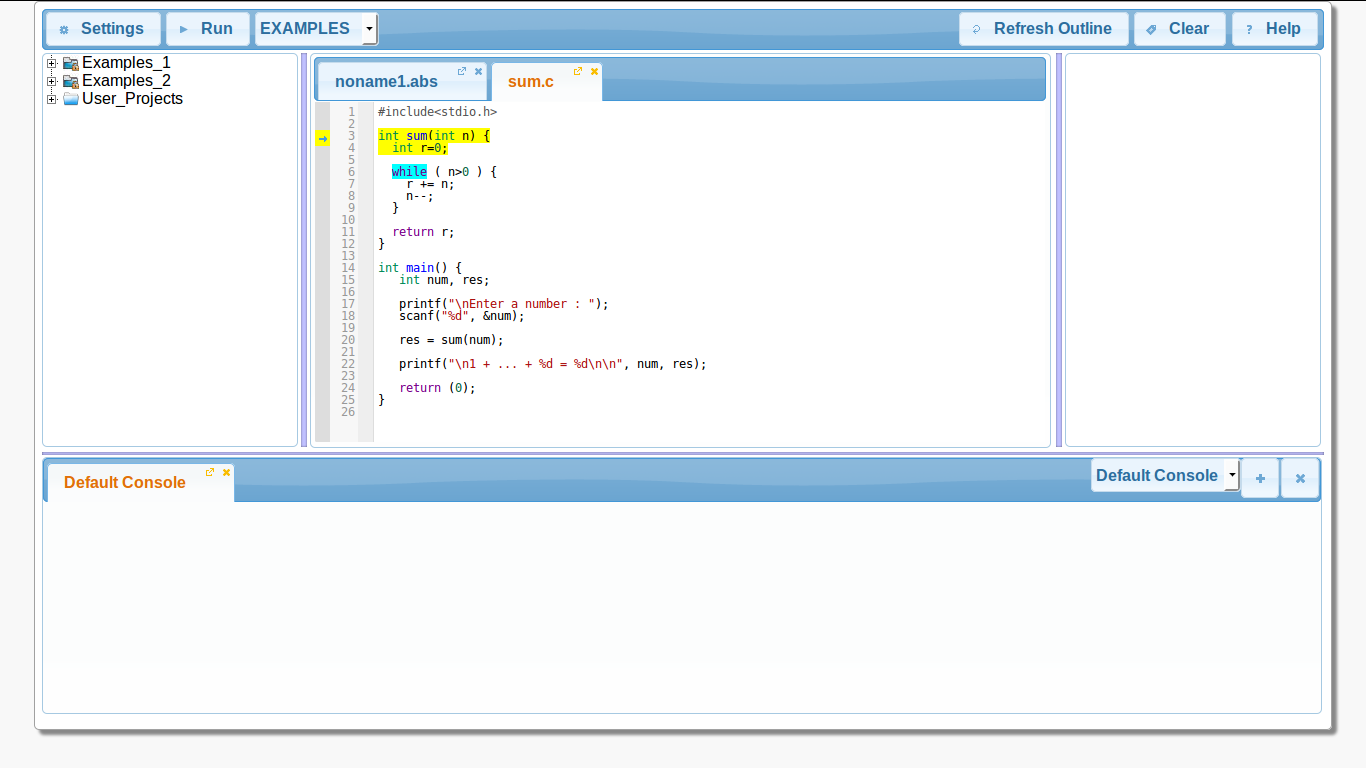
\includegraphics[width=1\textwidth]{fig/example2.png}
\end{center}
\caption{Output of Example~\ref{sec:eiol:examples:2}}
\label{fig:examples:2}
\hrule
\end{figure}
\end{example}


\begin{example}
\label{sec:eiol:examples:3}

The following is an example of \xmlstructref{eiout}{dialogboxcommand},
using a \xmlstructref{eiout}{content} environment with \lst{graph}
format.

\medskip
\begin{lstlisting}
<dialogbox boxtitle="CPU use" boxwidth="800" boxheight="500">
  <content format="graph">
    { "title":"BFS - Acer G5453",
      "f-titles":["Time","% CPU","% Mem"],
      "y-title":"%",
      "x-title":"Time",
      "groups":["BFS"],
      "labels":["Acer","G5453"],
      "values":[[1,22,43],[2,40,47],[3,82,88],[4,40,75]]
    }
    { "title":"BFS - Acer B12",
      "f-titles":["Timee","% CPU","% Mem"],
      "y-title":"%",
      "x-title":"Time",
      "groups":["BFS"],
      "labels":["Acer","B12"],
      "values":[[1,42,66],[2,65,47],[3,99,91],[4,68,92]]
    }
  </content>
</dialogbox>
\end{lstlisting}

\medskip
\noindent
Its execution in the web-client generates the output depicted in
Figure~\ref{fig:examples:3}.

\begin{figure}[h]
\hrule\smallskip
\begin{center}
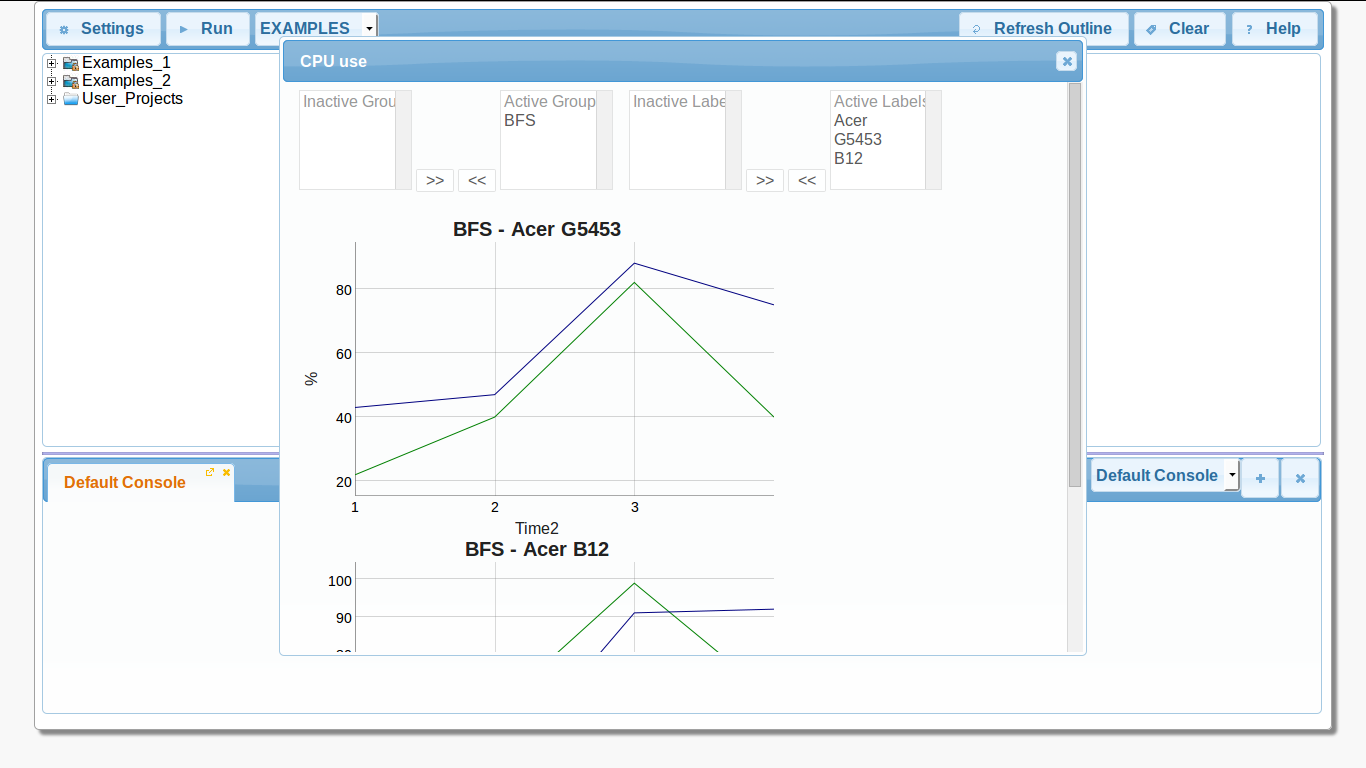
\includegraphics[width=1\textwidth]{fig/example3.png}
\end{center}
\caption{Output of Example~\ref{sec:eiol:examples:3}}
\label{fig:examples:3}
\hrule
\end{figure}

\begin{example}
\label{sec:eiol:examples:4}
%
The following is an example of \xmlstructref{eiout}{writefilecommand},
which adds a new file to the file-manager:

\medskip
\begin{lstlisting}
<writefile filename="dir1/newfile.cpp" overwrite="false">
<![CDATA[
#include <iostream>
using namespace std;
int main(){
  cout << "Hello World!" << endl;
  return 0;
}
]]>
</writefile>
\end{lstlisting}

\medskip
\noindent
Note the of \lst{<![CDATA[ ... ]]>}, this is necessary due to the use
of plain-text with special characters. Its execution in the web-client
generates the output depicted in Figure~\ref{fig:examples:4}.

\begin{figure}[h]
\hrule\smallskip
\begin{center}
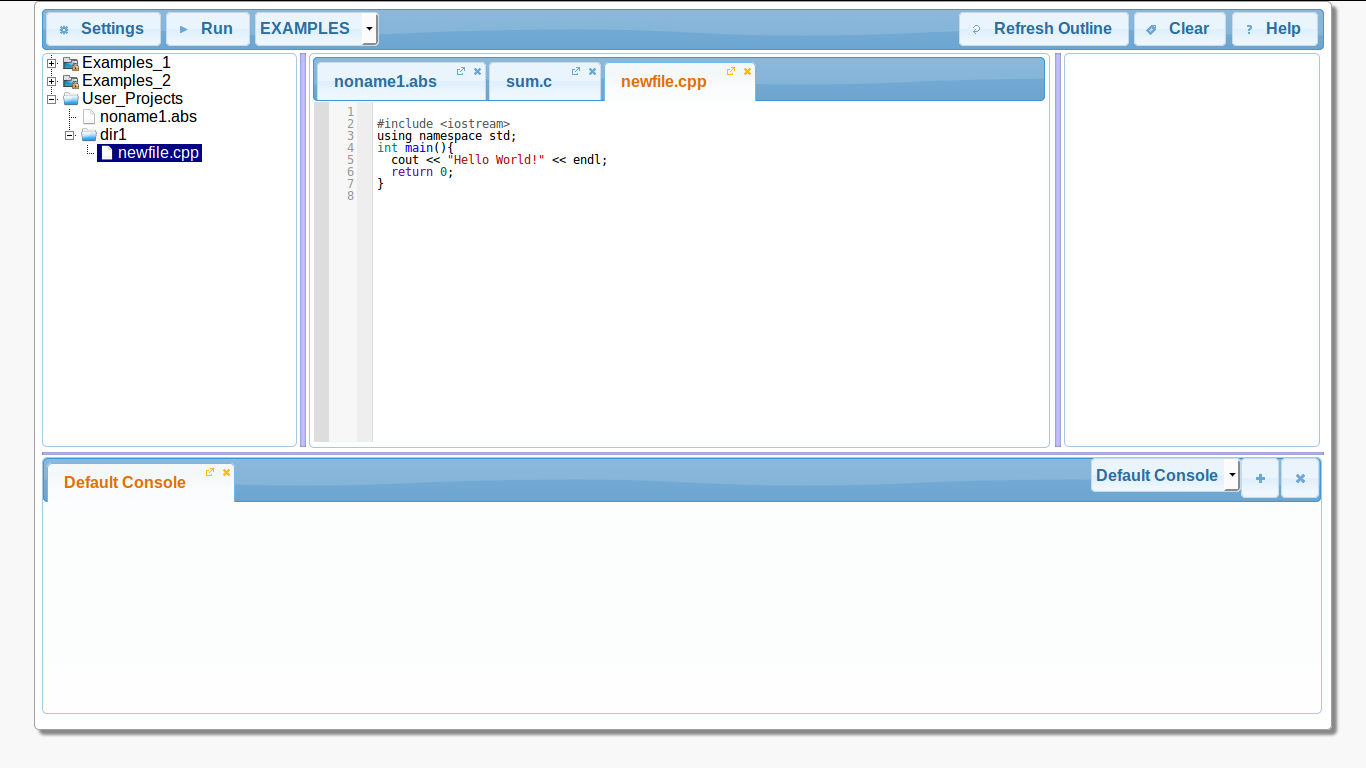
\includegraphics[width=1\textwidth]{fig/example4.png}
\end{center}
\caption{Output of Example~\ref{sec:eiol:examples:4}}
\label{fig:examples:4}
\hrule
\end{figure}
\end{example}

\end{example}

\begin{example}
\label{sec:eiol:examples:5}
%
The following is an example of \xmlstructref{eiout}{setcsscommand},
together with an action \xmlstructref{eiout}{onclickaction} which
changes the size of some text when it is clicked:

\medskip
\begin{lstlisting}
<eicommands>
 <printonconsole>
  <content format="html">
   <div id="wrap">
    <span>(*Some text*)</span><br/>
    <span id="text">Click me!</span><br/>
   </div> 
  </content>
 </printonconsole>
</eicommands>
<eiactions>
 <onclick>
  <elements>
   <selector value="#text" />
  </elements>
  <eicommands>
   <setcss>
    <elements>
     <selector value="#text" />
    </elements>
    <cssproperties>
     <cssproperty name="font-size" value="30px" />
    </cssproperties>
   </setcss>
  </eicommands>
 </onclick>
</eiactions>
\end{lstlisting}

\medskip
\noindent
Its execution in the web-client generates the output depicted in
Figure~\ref{fig:examples:5} -- it includes the result after clicking
on the text ``\lst{Click me!}''.

\begin{figure}[h]
\hrule\smallskip
\begin{center}
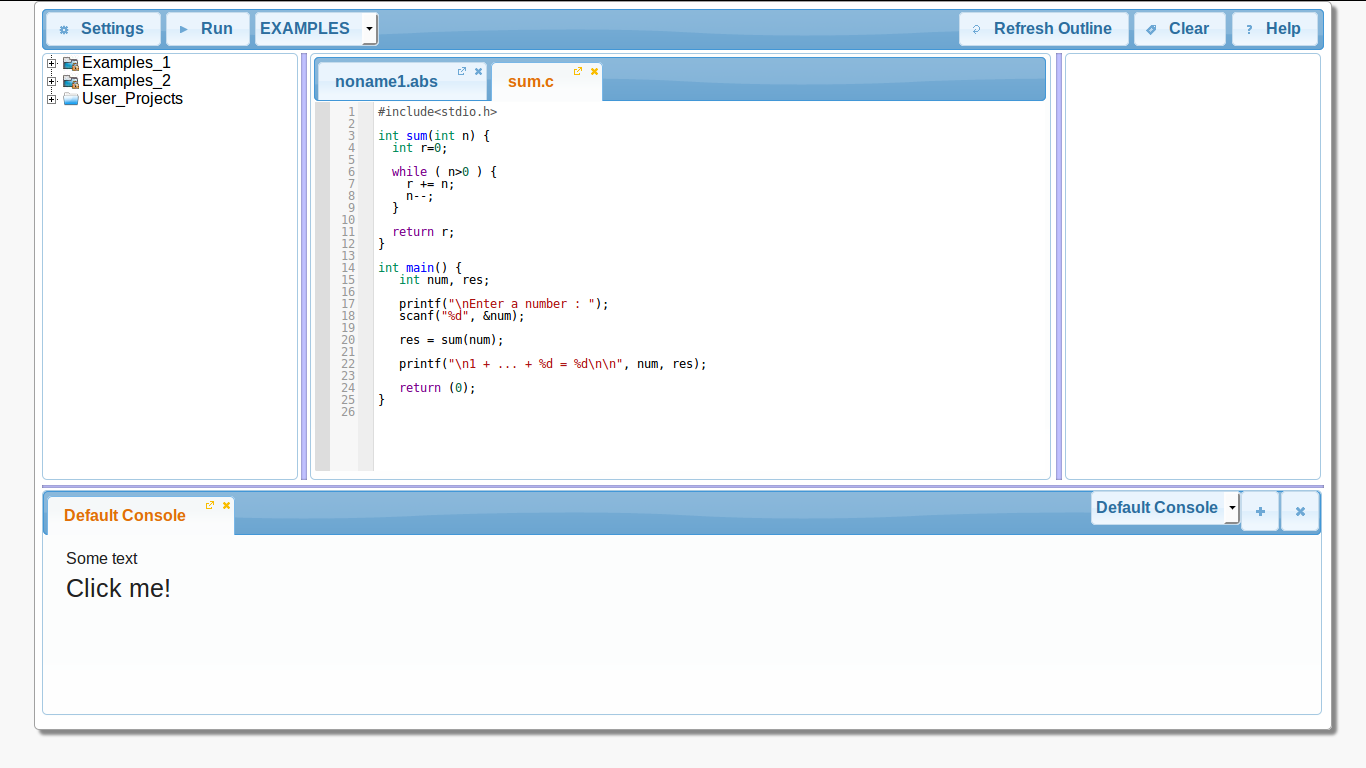
\includegraphics[width=1\textwidth]{fig/example5.png}
\end{center}
\caption{Output of Example~\ref{sec:eiol:examples:5}}
\label{fig:examples:5}
\hrule
\end{figure}
\end{example}

\begin{example}
\label{sec:eiol:examples:6}
%
The following is an example of
\xmlstructref{eiout}{changecontentcommand}. Assuming that we add the
following command to the list of commands of the
\xmlstructref{eiout}{onclickaction} in
Example~\ref{sec:eiol:examples:5}, it will add some text to the HTML
tag with identifier \lst{wrap} when ``\lst{Click me!}'' is clicked:

\medskip
\begin{lstlisting}
<changecontent action="append">
 <elements>
  <selector value="#wrap"/>
 </elements>
 <content format="html">
  <span style="color:red;">New Text added </span><br/>
 </content>
</changecontent> 
\end{lstlisting}

\medskip
\noindent
Its execution in the web-client generates the output depicted in
Figure~\ref{fig:examples:6} (after clicking on ``\lst{Click me!}'').

\begin{figure}[h]
\hrule\smallskip
\begin{center}
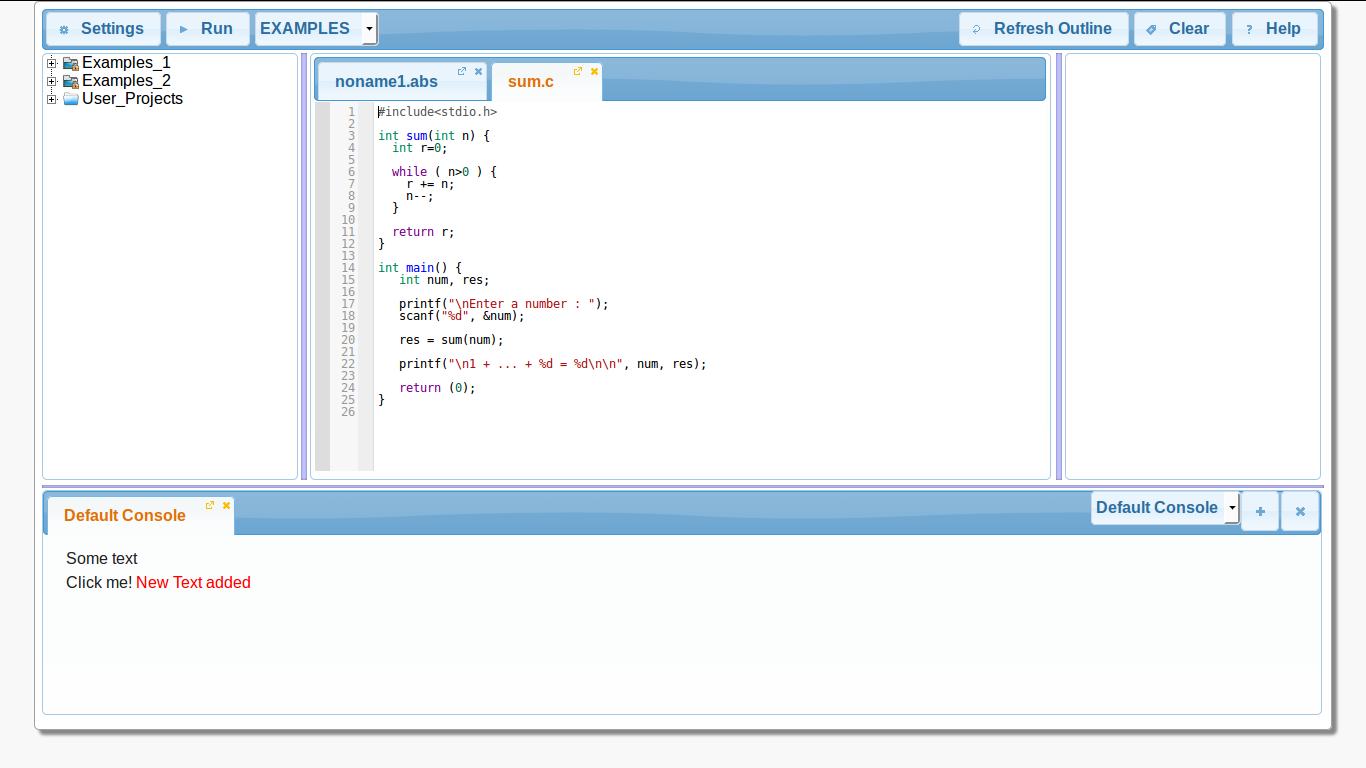
\includegraphics[width=1\textwidth]{fig/example6.png}
\end{center}
\caption{Output of Example~\ref{sec:eiol:examples:6}}
\label{fig:examples:6}
\hrule
\end{figure}
\end{example}

\begin{example}
\label{sec:eiol:examples:7}
%
The following is an example of \xmlstructref{eiout}{addmarkercommand},
using different \xmlstructattr{outclass} values:

\medskip
\begin{lstlisting}
<addmarker outclass="info">
 <lines>
  <line from="2" />
 </lines>
 <content format="text">
  Information
 </content>
</addmarker>
<addmarker outclass="warning">
 <lines>
  <line from="4" />
 </lines>
 <content format="text">
  Warning
 </content>
</addmarker>
<addmarker outclass="error">
 <lines>
  <line from="6" />
 </lines>
 <content format="text">
  Error
 </content>
</addmarker>
\end{lstlisting}

\medskip
\noindent
Its execution in the web-client generates the output depicted in
Figure~\ref{fig:examples:7}.

\begin{figure}[h]
\hrule\smallskip
\begin{center}
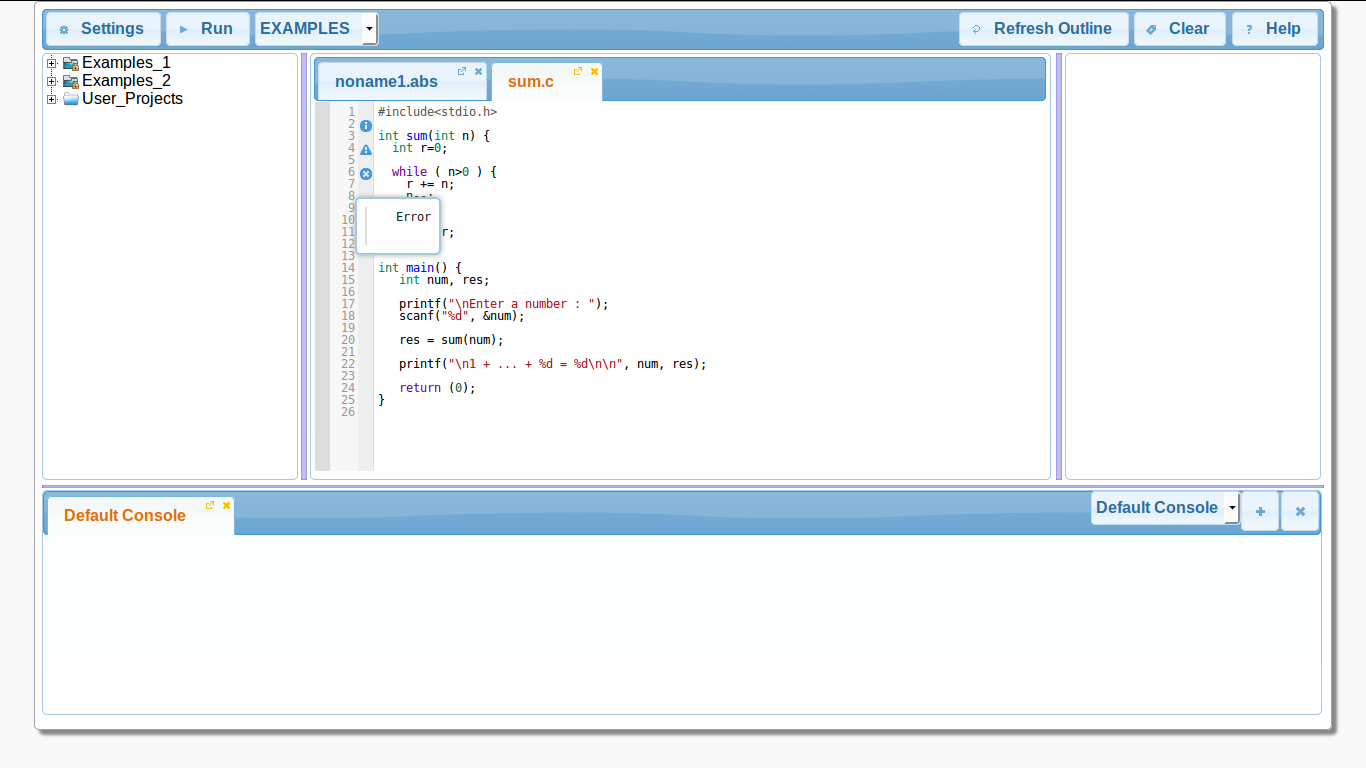
\includegraphics[width=1\textwidth]{fig/example7.png}
\end{center}
\caption{Output of Example~\ref{sec:eiol:examples:7}}
\label{fig:examples:7}
\hrule
\end{figure}
\end{example}

\begin{example}
\label{sec:eiol:examples:8}
%
The following is an example of 
\xmlstructref{eiout}{addinlinemarkercommand} using different
\xmlstructattr{outclass} values:

\medskip
\begin{lstlisting}
<addinlinemarker outclass="info">
 <lines>
  <line from="2" />
 </lines>
 <content format="text">
  Information
 </content>
</addinlinemarker>
<addinlinemarker outclass="warning">
 <lines>
  <line from="4" />
 </lines>
 <content format="text">
  Warning
 </content>
</addinlinemarker>
<addinlinemarker outclass="error">
 <lines>
  <line from="6" />
 </lines>
 <content format="text">
  Error
 </content>
</addinlinemarker>
\end{lstlisting}

\medskip
\noindent
Its execution in the web-client generates the output depicted in
Figure~\ref{fig:examples:8}.

\begin{figure}[h]
\hrule\smallskip
\begin{center}
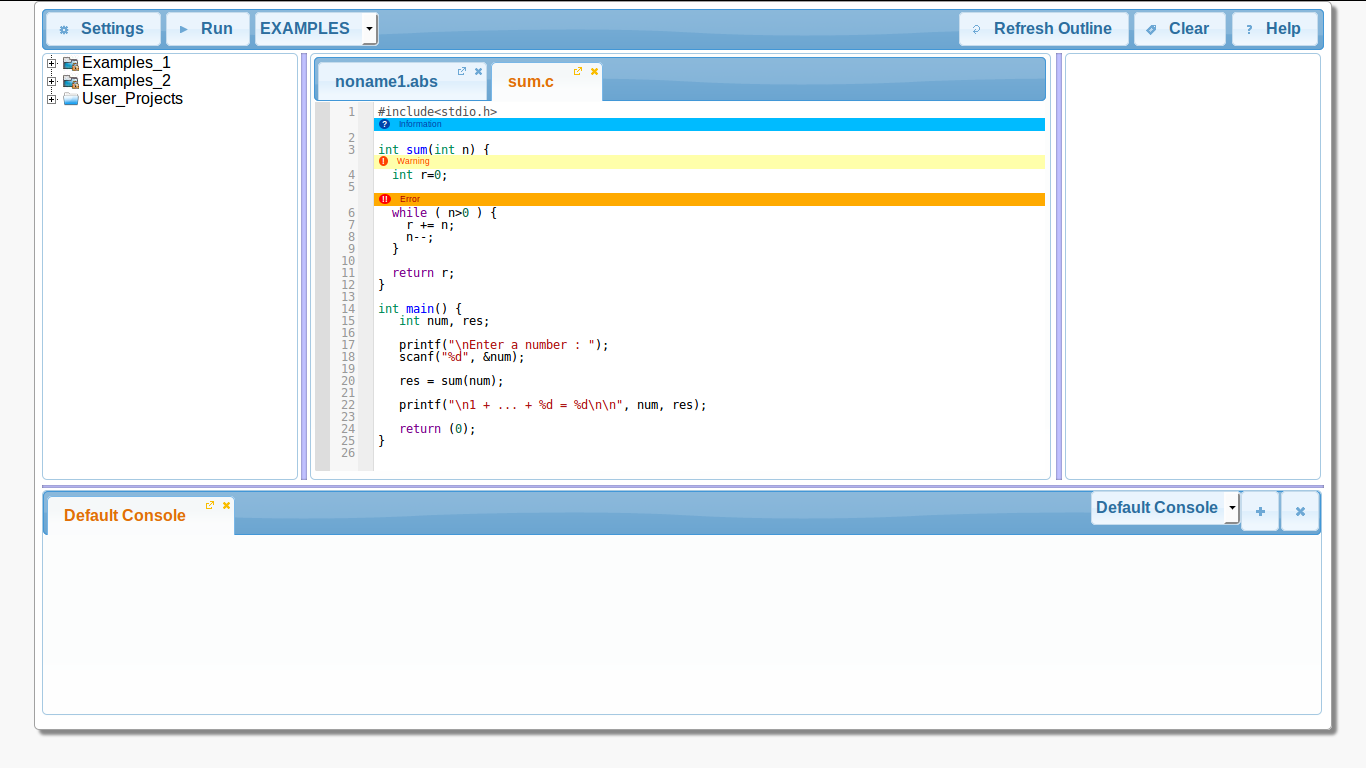
\includegraphics[width=1\textwidth]{fig/example8.png}
\end{center}
\caption{Output of Example~\ref{sec:eiol:examples:8}}
\label{fig:examples:8}
\hrule
\end{figure}
\end{example}

\begin{example}
\label{sec:eiol:examples:9}
%
The following is an example of \xmlstructref{eiout}{downloadcommand},
to download a file called \lst{$\mbox{download.test}$} generated by a
tool execution with \emph{execution identifier} \lst{xV54fga}:

\medskip
\begin{lstlisting}[mathescape=false]
<download execid="xV54fga" filename="download.test" />
\end{lstlisting}
%$
\medskip
\noindent
Its execution in the web-client generates the output as in
Figure~\ref{fig:examples:9}.

\begin{figure}[h]
\hrule\smallskip
\begin{center}
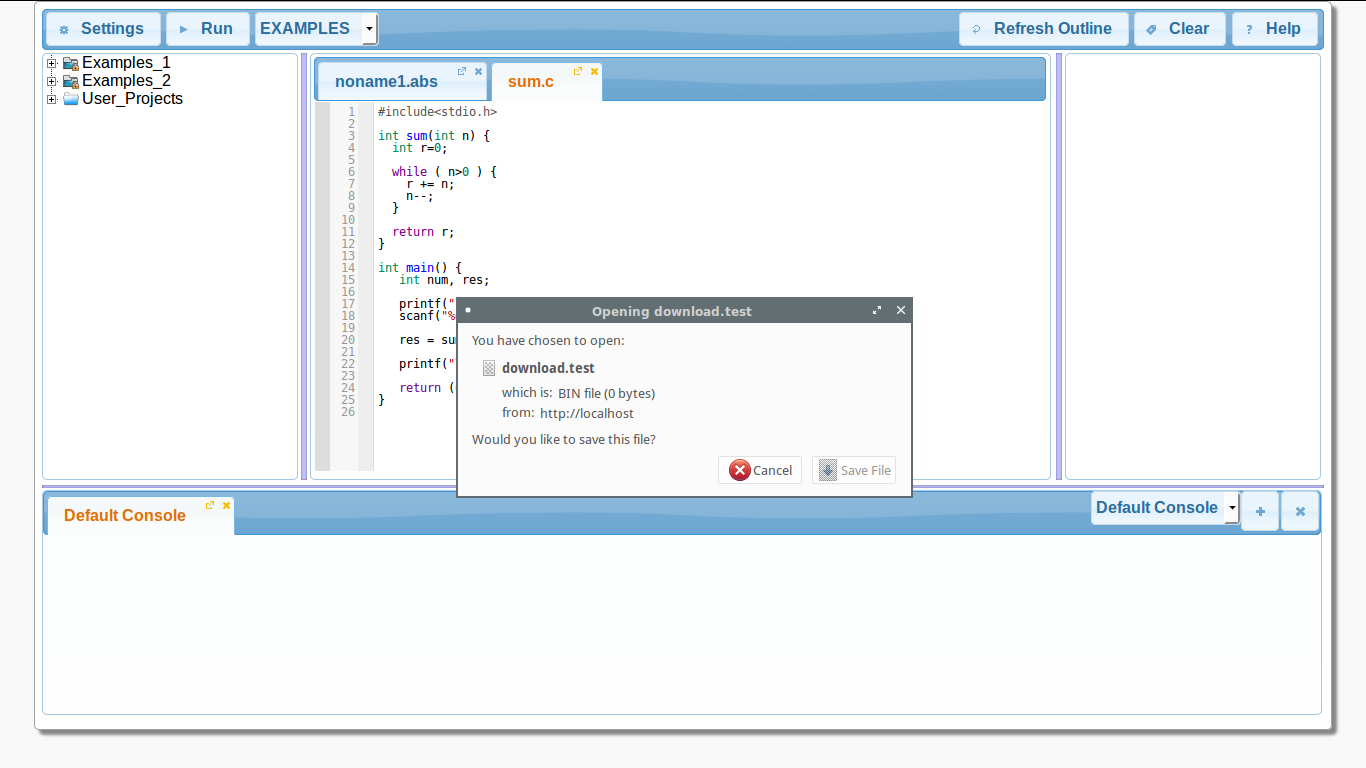
\includegraphics[width=1\textwidth]{fig/example9.png}
\end{center}
\caption{Output of Example~\ref{sec:eiol:examples:9}}
\label{fig:examples:9}
\hrule
\end{figure}
\end{example}




\end{document}

%%% Local Variables:
%%% mode: latex
%%% TeX-master: t
%%% End:
